% =====================================================================
%  The exploration, explained from the paper outward
%  Reply to the note of 13 August 2026.
%  Self-contained: no .bib, no \includegraphics, no external data.
%  Compiles on Overleaf as-is, and locally with:
%      tectonic -X compile reports/2026-08-19_discrepancy_explained.tex
% =====================================================================
\documentclass[11pt,a4paper]{article}

\usepackage[T1]{fontenc}
\usepackage[utf8]{inputenc}
\usepackage{lmodern}
\usepackage[margin=2.3cm]{geometry}
\usepackage{amsmath,amssymb}
\usepackage{booktabs}
\usepackage{array}
\usepackage{enumitem}
\usepackage{xcolor}
\usepackage{microtype}
\usepackage{caption}
\usepackage{tikz}
\usetikzlibrary{positioning,arrows.meta,calc,fit,backgrounds}
\usepackage{pgfplots}
\pgfplotsset{compat=1.18}

\definecolor{BlueLink}{HTML}{1F4E79}
\definecolor{BadRed}{HTML}{B3261E}
\definecolor{ModC}{HTML}{1F4E79}   % modularity family
\definecolor{LapC}{HTML}{2F6F4E}   % Laplacian family
\definecolor{CorrC}{HTML}{7A6A55}  % correlation family
\definecolor{ScalC}{HTML}{B3261E}  % the scalar Q
\definecolor{Panel}{HTML}{EDEFF2}
\definecolor{Panel2}{HTML}{F7F5F0}
\definecolor{Rule}{HTML}{9AA3AD}

\usepackage[colorlinks=true,linkcolor=BlueLink,urlcolor=BlueLink]{hyperref}
\emergencystretch=3em

\newcommand{\Q}{Q}
\newcommand{\Lap}{\mathbf{L}}
\newcommand{\Amat}{\mathbf{A}}
\newcommand{\Bmat}{\mathbf{B}}
\newcommand{\Cmat}{\mathbf{C}}
\newcommand{\dvec}{\mathbf{d}}

\captionsetup{font=small,labelfont=bf,width=.94\textwidth}
\setlist[itemize]{topsep=3pt,itemsep=2pt,parsep=0pt,leftmargin=1.3em}
\setlist[enumerate]{topsep=3pt,itemsep=2pt,parsep=0pt,leftmargin=1.8em}
\setlength{\parskip}{3pt}
\pagestyle{plain}

% a boxed aside
\newsavebox{\asidebox}
\newenvironment{aside}[1]
 {\par\vspace{2.5mm}\begin{lrbox}{\asidebox}%
  \begin{minipage}{\dimexpr\textwidth-16pt\relax}\small\textbf{#1}\par\vspace{1mm}}
 {\end{minipage}\end{lrbox}%
  \noindent\setlength{\fboxsep}{7pt}\setlength{\fboxrule}{.4pt}%
  \fcolorbox{Rule}{Panel2}{\usebox{\asidebox}}\par\vspace{2.5mm}}

\begin{document}

\begin{center}
{\Large\textbf{The exploration, explained from the paper outward}}\\[2mm]
{\normalsize Jash Dalal \quad$\cdot$\quad 19 August 2026}\\[1mm]
{\small Written in reply to the note of 13 August. Companion to
\texttt{reports/progress\_report.tex};\\ every number here is reproduced by the
scripts in \texttt{reports/probe/}.}
\end{center}
\vspace{2mm}
\hrule
\vspace{4mm}

\section*{Introduction}
\addcontentsline{toc}{section}{Introduction}

The note of 13 August asked two questions of my 12 August log entries: what
the key discrepancy is, and what directions follow from it. Those entries state
their conclusions without building up to them, which is fair criticism. This
document is the chain that leads to them, starting from the definitions in the
papers themselves. This introduction gives the whole argument in outline --- the
three papers it rests on, what appears to be wrong and why, how each of those
things was checked, and what came out --- and every claim in it is built up from
first principles later on.

\subsection*{The three papers}

Three papers were replicated in full before any of this began; they were treated
as a literature review rather than as ends in themselves. Two of them supply the
crisis indicators that this exploration compares.

\begin{center}\small
\renewcommand{\arraystretch}{1.22}\setlength{\tabcolsep}{4.5pt}
\begin{tabular}{@{}>{\raggedright\arraybackslash}p{3.55cm}
                  >{\raggedright\arraybackslash}p{4.95cm}
                  >{\raggedright\arraybackslash}p{2.4cm}
                  >{\raggedright\arraybackslash}p{4.4cm}@{}}
\toprule
\textbf{Paper} & \textbf{What it builds} & \textbf{Its indicator} &
\textbf{How the rebuild came out} \\
\midrule
\textbf{Paper 1.} Cardoso \& Palomar (2020), \emph{Learning Undirected Graphs
in Financial Markets} &
Learns a graph Laplacian $\Lap$ \emph{directly} from returns by penalised
maximum likelihood under a Gaussian Markov random field --- no correlation
table, no threshold. &
$\lambda_2(\Lap)$, the \textbf{Fiedler value}: how tightly the graph holds
together. Small means close to falling apart. &
The method, the monthly path of $\lambda_2$ and the COVID exit all reproduce.
The trading result does not: the strategy ends at $-0.011$ where buy-and-hold
ends at $+0.078$, with no threshold moved to rescue it. \\
\addlinespace[2pt]
\textbf{Paper 2.} Hallac, Vare, Boyd \& Leskovec (2017), \emph{TICC} &
Cuts a multivariate series into stretches, each with its own block-Toeplitz
dependence pattern, so a regime can recur later. Not a network method. &
None --- it labels regimes rather than scoring days. &
Headline accuracy reproduces; the ablations come out weaker than reported, so
the rebuild makes the method look \emph{more} necessary than the paper does.
Peripheral here, but the only one modelling a state that persists in time. \\
\addlinespace[2pt]
\textbf{Paper 3.} Silva et al.\ (2015), \emph{Modular Dynamics of Financial
Market Networks} &
One network per day: keep the strongest $10\%$ of pairwise correlations as
edges, run Louvain, record how cleanly the stocks split into groups.
6{,}315 daily networks, 360 stocks, 25 years. &
$\Q(t)$, \textbf{modularity}: a single number per day for how group-like the
market is. &
Reproduces on its own terms. What the number \emph{means} is the problem, and
that is this document's subject. A separate 26-item audit of it is already on
file. \\
\bottomrule
\end{tabular}
\end{center}

\noindent The prompt behind this work (\S1) was to put Paper 1's indicator and
Paper 3's side by side, and to look at the \textbf{modularity matrix} --- the
matrix $\Q$ is computed from --- rather than only at $\Q$ itself. Papers 1 and 3 therefore
supply the two candidates; Paper 2 sits to one side as a possible comparator.

\subsection*{What appears to be wrong, and what would explain it}

Five things came out of the exploration that do not fit the papers' own account
of themselves. The middle column is a candidate explanation, not a settled one;
the last says where the reasoning is set out in full.

\begin{center}\small
\renewcommand{\arraystretch}{1.22}\setlength{\tabcolsep}{4.5pt}
\begin{tabular}{@{}>{\raggedright\arraybackslash}p{5.7cm}
                  >{\raggedright\arraybackslash}p{8.05cm}
                  >{\raggedright\arraybackslash}p{1.3cm}@{}}
\toprule
\textbf{What was observed} & \textbf{What would explain it} & \textbf{Where} \\
\midrule
$\Q(t)$ barely separates crisis days from calm ones (AUC $0.538$, coin flip
$0.500$), while three other readings of \emph{the same} matrix reach $0.722$ to
$0.760$. &
The reduction, not the matrix. $\Q$ collapses $129{,}600$ matrix entries to
about nine groups to one number; almost everything is discarded on the way. The
discarded threshold $\tau(t)$ alone scores $0.807$. &
\S5 \\
\addlinespace[2pt]
Louvain reports a median of \emph{nine} communities every day, yet i.i.d.\
Gaussian noise pushed through the identical pipeline scores $\Q=0.2246$ against
the real market's $0.2215$. &
Thresholding a correlation matrix yields a triangle-rich, transitive graph by
construction, and such graphs always look modular. The partition may be an
artifact of the construction rather than a property of the market. &
\S6.2 \\
\addlinespace[2pt]
At a 30-day window on 360 stocks, the average number of correlation eigenvalues
escaping the random-matrix noise band is $\mathbf{0.70}$, and zero on $2{,}668$
of $6{,}315$ days. &
The window is too short for the question. Thirty observations give a
correlation matrix of rank at most $29$, so most of what is called community
structure is not statistically resolvable at the window length this literature
itself uses. &
\S6.3 \\
\addlinespace[2pt]
Theory makes the two indicators one number --- $\lambda_2(\Lap)+\mu_1(\Bmat)=d$
on a $d$-regular graph, and Silva pins the mean degree at $35.90$ daily --- but
the measured sum is $26.41$, and the two correlate at $-0.187$ where the
identity demands $-1$. &
The identity's premises fail in three separable ways: degree heterogeneity
(fixed \emph{average} degree is not a regular graph), fragmentation (these
networks are disconnected on $63\%$ of days), and the market mode. Which of the
three carries the crisis information is an open, answerable question. &
\S7 \\
\addlinespace[2pt]
The three highest-scoring detectors correlate above $0.99$ with each other, and
every variable added to them helps in-sample while hurting out-of-sample on a
strict pre/post-2002 split. &
They are one signal, not three: the market mode, published as the absorption
ratio in 1999. The in/out-of-sample gap is the textbook overfitting signature,
though $27$ test events is too few to settle it. &
\S8 \\
\bottomrule
\end{tabular}
\end{center}

\subsection*{How each of those was checked}

Nothing above rests on a new pipeline. Silva's replication already builds one
network per day for 6{,}315 days, and each check reuses it unchanged so that
old and new numbers are directly comparable.

\begin{itemize}
\item \textbf{One ruler for everything} (\S4). Every candidate is turned into a
250-day trailing $z$-score computed on strictly prior data, then scored by AUC
against crisis windows fixed in advance ($17$ events, $2.68\%$ base rate). As a
control the probe re-derives Silva's own stored $\Q$ and $\tau$ scores to ten
decimal places, so the new numbers sit on exactly the ruler the old ones do.
\item \textbf{Full spectra rather than one statistic.} All eigenvalues of three
operators --- the Laplacian $\Lap$, the modularity matrix $\Bmat$ and the
correlation matrix $\Cmat$ --- on each of the 6{,}315 networks, with every
resulting statistic scored on that same ruler. This is what makes the
matrix-versus-scalar comparison a measurement rather than an argument.
\item \textbf{The identity tested directly}, and then re-tested on the largest
connected component only, which removes fragmentation as a confound and lets
its contribution be separated from the rest.
\item \textbf{Matched nulls taken from the replication itself}: i.i.d.\
Gaussian returns through the identical construction, and Louvain re-run across
ten seeds to measure how much of the daily variation in $\Q$ is the algorithm
rather than the market.
\item \textbf{Incremental value, in-sample and out.} Whether the modularity
spectrum adds anything to the market mode, judged both in-sample and on a
strict chronological split at 2002.
\item \textbf{Arithmetic re-derived.} A checking script recomputes all $91$
values quoted in this document from the stored artifacts and confirms each
printed string appears in the source, so the prose cannot drift from the data
in either direction (Appendix~A).
\end{itemize}

\subsection*{Summary}

\begin{aside}{The discrepancy, in one sentence.}
Silva et al.\ reduce a $360\times360$ matrix to a single number $\Q(t)$; that
number is almost uninformative about crises (AUC $0.538$, against $0.500$ for a
coin), while three other readings of \emph{the same matrix, on the same
networks, under the same test} score $0.722$ to $0.760$ --- so the information
was present, and the reduction is where it was lost. \hfill(\S5)
\end{aside}

\noindent That is the answer to the first question. Around it sit a second,
structural discrepancy --- the two candidate indicators are provably the same
number and empirically unrelated (\S7) --- and one finding that cuts against the
whole exercise: at the window length in use there may be very little community
structure to detect in the first place (\S6.3). The strongest detectors, mean\-while,
are one already-known signal, and nothing yet beats it out of sample (\S8).

On the second question, three directions follow. They are set out in \S9 in a
common frame, at equal length, with no ordering implied and no combined
recommendation.

\begin{itemize}
\item \textbf{D1} --- decompose the $9.49$ residual into its degree, fragmentation
and market-mode parts, and compare the Laplacian and modularity families as one
structural question rather than as a leaderboard.
\item \textbf{D2} --- map where on the (window length, universe size, density)
grid community detection in correlation networks is statistically possible at
all, and replace the Louvain community count with a deterministic one.
\item \textbf{D3} --- the negative end of the modularity spectrum:
anti-communities, groups trading against each other, which thresholding
structurally cannot see.
\end{itemize}

\noindent Appendix~A lists where every number quoted above comes from and how to
re-derive it.

\section{Where the question came from}

The question was not what those three papers claim --- that is settled in the
replications --- but what to build on top of them. That question came from my
supervisor:

\begin{quote}\itshape
Paper 1's crash indicator is the Fiedler value $\lambda_2(\Lap)$. Paper 3's is
modularity $\Q$. Look at the \textbf{modularity matrix} as well --- its
eigenvalues and singular values may carry more. Can we get a study out of
comparing Laplacian against modularity matrices?
\end{quote}

Three things were done in response.

\textbf{The repository was re-read end to end} --- the three pipelines
summarised in the introduction, together with the 26-item methodological audit
already run against Silva.

\textbf{The outside literature was searched} on two fronts: spectral
market-stress indicators in finance, and the mathematics of the modularity
matrix. The mathematics lives almost entirely outside finance --- MacMahon \&
Garlaschelli on the correct random-matrix null for correlation-based modularity,
Fasino \& Tudisco on the modularity spectrum and anti-communities, Nadakuditi \&
Newman on when community detection is possible at all. In finance, modularity
appears essentially only as the scalar $\Q$. Repeated searches for
modularity-matrix \emph{spectra} used as financial indicators returned nothing.

\begin{aside}{How far this search actually went.}
Not far, and I want to be straight about it. This survey was done largely
\emph{with} Claude rather than by reading the papers through: I used it to find
the relevant work, to summarise what each result says, and to check that no
existing paper already does what \S9 proposes. I have read abstracts, the
statements of the main results, and enough of MacMahon \& Garlaschelli and
Fasino \& Tudisco to use their results here --- but I have not worked through
the proofs, and I have not audited the finance side for papers the searches
missed. So treat the claim ``nobody in finance has used the modularity
\emph{spectrum}'' as a well-supported absence of evidence, not as a settled
literature review. It needs a proper one before it is put in writing anywhere
that matters.
\end{aside}

\textbf{Rather than speculate about what the modularity matrix would show, it
was computed.} Silva's pipeline already builds one network per day for 6{,}315
days. The probe takes the full spectrum of three operators on each of those
networks and scores every resulting statistic through the replication's
\emph{own} crisis detector --- reproducing the replication's stored scores to
ten decimal places as a control, so the new numbers sit on exactly the ruler the
old ones do.

The rest of this document is that chain, in order: what Silva computes (\S2),
what matrix sits underneath it (\S3), how anything gets scored (\S4), what came
out (\S5--\S8), and what could be done next (\S9).

\section{What Silva et al.\ actually compute}
\label{sec:pipeline}

Everything below is the replication's own code path
(\texttt{net/construct.py} in the Paper-3 tree), at full scale: 360 NYSE
common stocks, January 1986 to February 2011.

\textbf{Step 1 --- returns.} Daily log returns on adjusted closes,
$Y_i(t)=\ln P_i(t)-\ln P_i(t-1)$. A $360\times6{,}344$ panel.

\textbf{Step 2 --- a correlation matrix per day.} Slide a $\Delta t=30$ trading-day
window forward one day at a time. In each window, standardise each stock's
returns and form the $360\times360$ Pearson correlation matrix $\Cmat(t)$. That
is $\binom{360}{2}=\mathbf{64{,}620}$ pairwise correlations, each a real number
in $[-1,1]$. Sliding to the end of the panel gives \textbf{6{,}315} of these.

\textbf{Step 3 --- threshold to a graph.} Keep only the strongest correlations.
Crucially the threshold is \emph{not} fixed: each day $\tau(t)$ is re-solved so
that exactly $10\%$ of pairs survive,
\[
  A_{ij}(t)=\Theta\!\left(\rho_{ij}(t)-\tau(t)\right)-\delta_{ij},
  \qquad
  \#\{\text{edges}\}=0.10\cdot\tbinom{360}{2}=\mathbf{6{,}462}\ \ \text{every day.}
\]
Two consequences worth holding onto. First, $2m=12{,}924$ and the average degree
is $12{,}924/360=\mathbf{35.90}$ --- \emph{exactly}, every day, by construction,
not approximately. Second, $\tau(t)$ itself is a real quantity that varies a lot
(mean $0.444$, max $0.861$ on Black Monday); the pipeline computes it, uses it,
and discards it.

\textbf{Step 4 --- communities.} Run Louvain on the resulting graph. It returns a
partition of the 360 stocks into groups --- a median of 9 of them, though on
1987-10-19 it returns 156, of which 152 are single stocks.

\textbf{Step 5 --- one number.} Score that partition with Newman's modularity,
\[
  \Q=\sum_{c}\left[\frac{e_c}{m}-\left(\frac{d_c}{2m}\right)^{\!2}\right],
\]
and record it. $\Q(t)$ is the paper's central quantity; its 25-year trajectory is
the paper's story.

\begin{figure}[t]
\centering
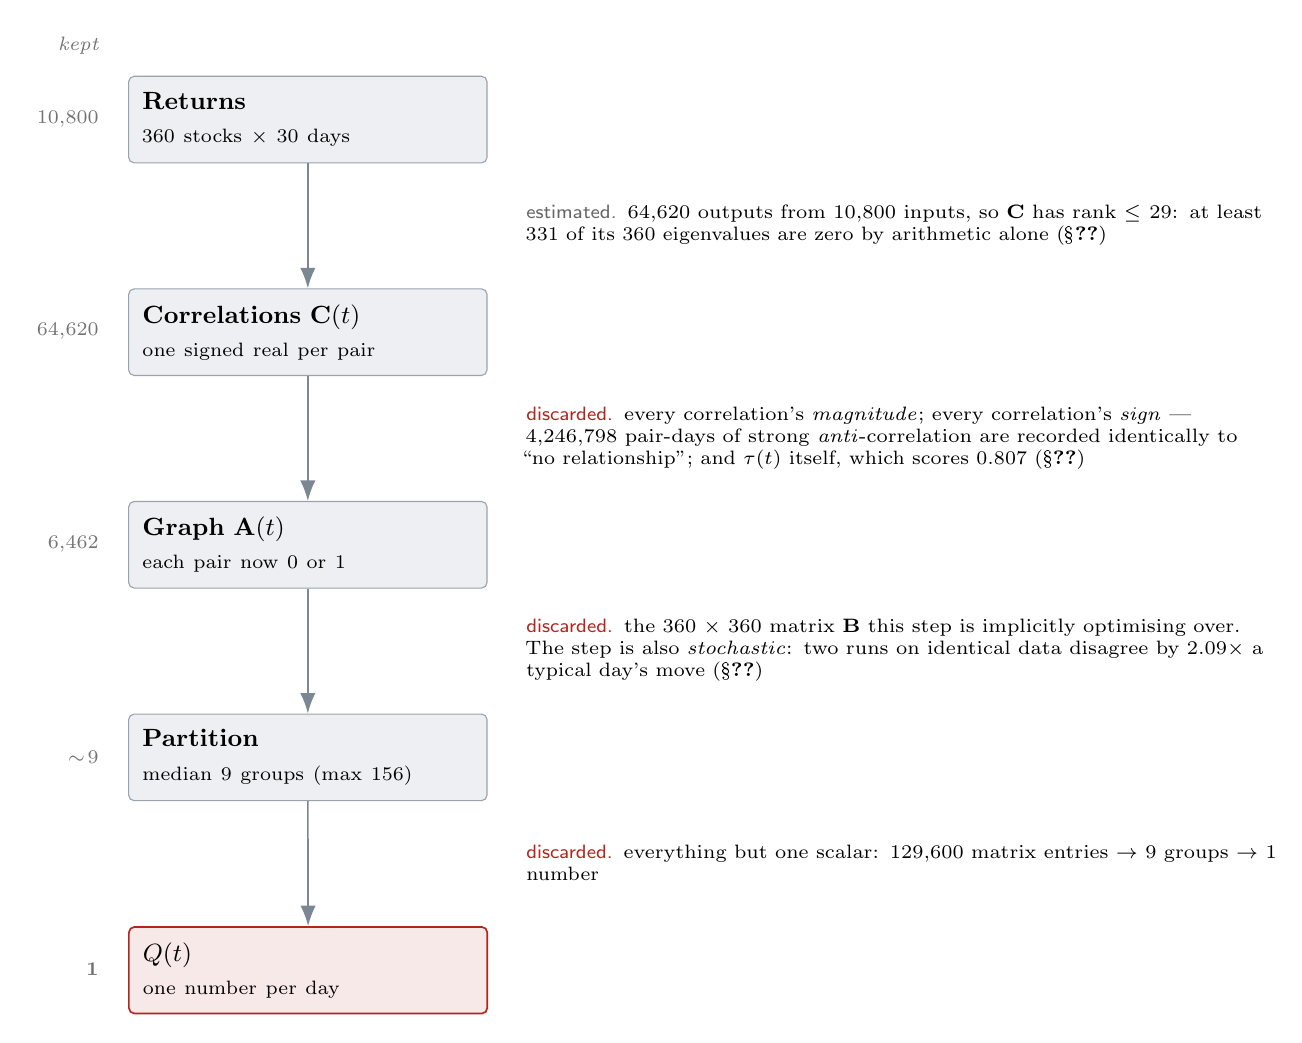
\begin{tikzpicture}[
  font=\small, x=1cm, y=1cm,
  box/.style={draw=Rule,line width=.4pt,rounded corners=2pt,fill=Panel,
              text width=42mm,align=left,inner sep=5pt,minimum height=11mm,
              anchor=north west},
  arr/.style={-{Latex[length=2.6mm]},line width=.6pt,draw=Rule!130},
  note/.style={text width=95mm,align=left,font=\scriptsize,anchor=west,
               inner sep=0pt},
  tag/.style={font=\scriptsize,color=black!55,anchor=east}]

\node[box] (r) at (0,0)
  {\textbf{Returns}\\[1pt]\scriptsize $360$ stocks $\times$ $30$ days};
\node[box] (c) at (0,-2.7)
  {\textbf{Correlations} $\Cmat(t)$\\[1pt]\scriptsize one signed real per pair};
\node[box] (a) at (0,-5.4)
  {\textbf{Graph} $\Amat(t)$\\[1pt]\scriptsize each pair now $0$ or $1$};
\node[box] (p) at (0,-8.1)
  {\textbf{Partition}\\[1pt]\scriptsize median $9$ groups (max $156$)};
\node[box,fill=ScalC!10,draw=ScalC,line width=.6pt] (q) at (0,-10.8)
  {\textbf{$\Q(t)$}\\[1pt]\scriptsize one number per day};

\node[font=\scriptsize\itshape,color=black!55,anchor=south east] at (-0.25,0.15) {kept};
\node[tag] at (-0.25,-0.55)  {$10{,}800$};
\node[tag] at (-0.25,-3.25)  {$64{,}620$};
\node[tag] at (-0.25,-5.95)  {$6{,}462$};
\node[tag] at (-0.25,-8.65)  {$\sim\!9$};
\node[tag] at (-0.25,-11.35) {$\mathbf{1}$};

\draw[arr] (r.south) -- (c.north);
\draw[arr] (c.south) -- (a.north);
\draw[arr] (a.south) -- (p.north);
\draw[arr] (p.south) -- (q.north);

\node[note] at (5.05,-1.9) {\textcolor{black!60}{\textsf{estimated.}}
  $64{,}620$ outputs from $10{,}800$ inputs, so $\Cmat$ has rank $\le29$:
  at least $331$ of its $360$ eigenvalues are zero by arithmetic alone\ (\S\ref{sec:mech})};
\node[note] at (5.05,-4.6) {\textcolor{BadRed}{\textsf{discarded.}} every
  correlation's \emph{magnitude}; every correlation's \emph{sign} ---
  $4{,}246{,}798$ pair-days of strong \emph{anti}-correlation are recorded
  identically to ``no relationship''; and $\tau(t)$ itself, which scores
  $0.807$\ (\S\ref{sec:disc})};
\node[note] at (5.05,-7.3) {\textcolor{BadRed}{\textsf{discarded.}} the
  $360\times360$ matrix $\Bmat$ this step is implicitly optimising over. The
  step is also \emph{stochastic}: two runs on identical data disagree by
  $2.09\times$ a typical day's move\ (\S\ref{sec:mech})};
\node[note] at (5.05,-10.0) {\textcolor{BadRed}{\textsf{discarded.}} everything
  but one scalar: $129{,}600$ matrix entries $\rightarrow$ $9$ groups
  $\rightarrow$ $1$ number};
\end{tikzpicture}
\caption{Silva's pipeline as a sequence of reductions; the right-hand column is
what each arrow costs. The paper reports the bottom box. The exploration in this
document consists entirely of asking what is in the boxes above it, and scoring
those contents on the paper's own ruler.}
\label{fig:pipeline}
\end{figure}

Figure~\ref{fig:pipeline} draws that chain with what each step throws away.
Nothing in it is a criticism yet --- every pipeline discards something, and a
scalar indicator is the point of the exercise. The question \S5 answers is
whether \emph{this particular} discard was expensive, and it is answerable
because the discarded objects can simply be scored too.

\section{The matrix underneath \texorpdfstring{$\Q$}{Q}}
\label{sec:matrix}

$\Q$ is not a primitive quantity. It is a summary of a specific matrix, and that
matrix is the object the prompt was about. This section builds it from
scratch.

\subsection{The question modularity is really asking}

Suppose stocks $i$ and $j$ have an edge. Is that interesting? Not necessarily.
If $i$ is connected to 200 of the other 359 stocks, an edge to $j$ says
almost nothing --- $i$ is connected to nearly everyone. But if $i$ and $j$ each
have only five edges and one of them is to each other, that is meaningful.

So a baseline is needed: \emph{how many edges would we expect between $i$ and
$j$ purely by accident, given how many edges each of them has?} Writing $d_i$
for the degree of stock $i$ (its number of edges) and $2m$ for the total number
of edge endpoints, the standard answer --- the configuration model --- is
\[
  \mathbb{E}\left[A_{ij}\right] \;=\; \frac{d_i d_j}{2m}.
\]
The intuition is a matching argument: stock $i$ has $d_i$ endpoints dangling,
each picks a partner at random from the $2m$ endpoints in the network, and $d_j$
of those belong to $j$.

Check it on the real numbers, where $2m=12{,}924$. Two typical stocks, each of
degree $36$:
\[
  \frac{36\times36}{12{,}924}=0.100,
\]
a $10\%$ chance --- exactly the density of the network, as it must be. Now two
hubs, each of degree $100$:
\[
  \frac{100\times100}{12{,}924}=0.774.
\]
Those two are expected to be connected almost certainly, just from being
popular. An edge between them is not news.

\subsection{The modularity matrix}

The \textbf{modularity matrix} is what was observed minus what chance predicts:
\[
  \Bmat \;=\; \Amat - \frac{\dvec\dvec^{\!\top}}{2m},
  \qquad
  B_{ij}=A_{ij}-\frac{d_id_j}{2m}.
\]
It is the same size as $\Amat$, $360\times360$, and every entry is a surprise
score. Table~\ref{tab:surprise} reads off the four cases using the real numbers
just computed.

\begin{table}[h]
\centering\small
\caption{Entries of $\Bmat$ as surprise scores, using the two expectations
computed above. The last row is the one to keep hold of.}
\label{tab:surprise}
\begin{tabular}{@{}llrl@{}}
\toprule
observed & expected & $B_{ij}$ & reading \\
\midrule
edge ($1$)    & $0.10$ & $+0.90$ & strong surprise: together far more than chance \\
edge ($1$)    & $0.77$ & $+0.23$ & two hubs linked; barely news \\
no edge ($0$) & $0.10$ & $-0.10$ & ordinary; most pairs look like this \\
no edge ($0$) & $0.77$ & $\mathbf{-0.77}$ & two hubs \emph{avoiding} each other \\
\bottomrule
\end{tabular}
\end{table}

That last row is the structural point. $\Bmat$ has a meaningful negative end: it
can say \emph{``an edge should be here and is not.''} The adjacency matrix is
$0/1$ and the Laplacian is built from $\Amat$ and the degrees, so
\textbf{neither can express that}. The asymmetry is real, and it is where
direction D3 comes from.

Figure~\ref{fig:bmatrix} shows the subtraction on a small graph where the
arithmetic can be checked by eye.

\begin{figure}[t]
\centering
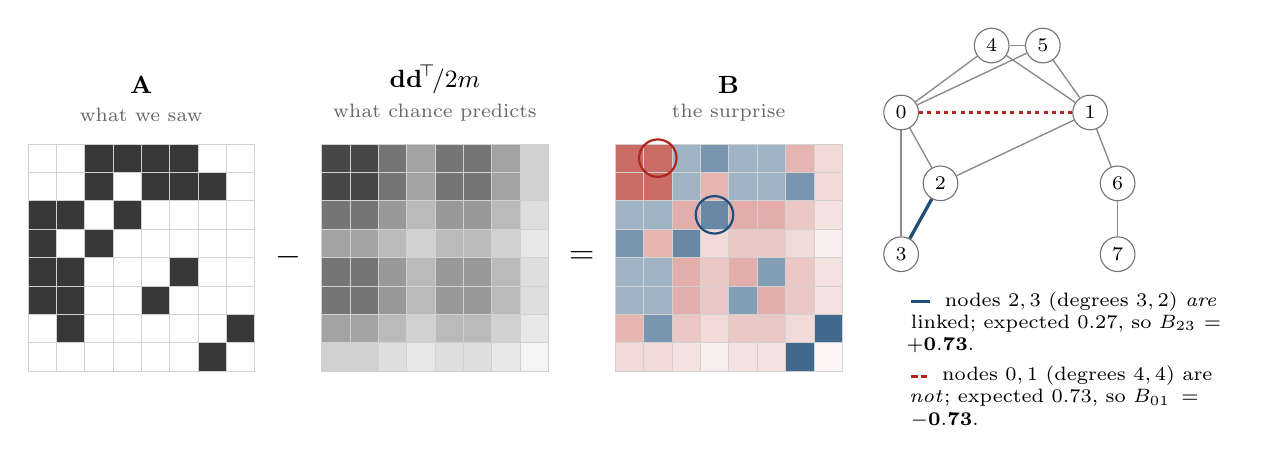
\begin{tikzpicture}[font=\small,x=1cm,y=1cm]
\fill[white,draw=black!18,line width=.15pt] (0.000,0.000) rectangle ++(0.360,-0.360);
\fill[white,draw=black!18,line width=.15pt] (0.360,0.000) rectangle ++(0.360,-0.360);
\fill[black!78,draw=black!18,line width=.15pt] (0.720,0.000) rectangle ++(0.360,-0.360);
\fill[black!78,draw=black!18,line width=.15pt] (1.080,0.000) rectangle ++(0.360,-0.360);
\fill[black!78,draw=black!18,line width=.15pt] (1.440,0.000) rectangle ++(0.360,-0.360);
\fill[black!78,draw=black!18,line width=.15pt] (1.800,0.000) rectangle ++(0.360,-0.360);
\fill[white,draw=black!18,line width=.15pt] (2.160,0.000) rectangle ++(0.360,-0.360);
\fill[white,draw=black!18,line width=.15pt] (2.520,0.000) rectangle ++(0.360,-0.360);
\fill[white,draw=black!18,line width=.15pt] (0.000,-0.360) rectangle ++(0.360,-0.360);
\fill[white,draw=black!18,line width=.15pt] (0.360,-0.360) rectangle ++(0.360,-0.360);
\fill[black!78,draw=black!18,line width=.15pt] (0.720,-0.360) rectangle ++(0.360,-0.360);
\fill[white,draw=black!18,line width=.15pt] (1.080,-0.360) rectangle ++(0.360,-0.360);
\fill[black!78,draw=black!18,line width=.15pt] (1.440,-0.360) rectangle ++(0.360,-0.360);
\fill[black!78,draw=black!18,line width=.15pt] (1.800,-0.360) rectangle ++(0.360,-0.360);
\fill[black!78,draw=black!18,line width=.15pt] (2.160,-0.360) rectangle ++(0.360,-0.360);
\fill[white,draw=black!18,line width=.15pt] (2.520,-0.360) rectangle ++(0.360,-0.360);
\fill[black!78,draw=black!18,line width=.15pt] (0.000,-0.720) rectangle ++(0.360,-0.360);
\fill[black!78,draw=black!18,line width=.15pt] (0.360,-0.720) rectangle ++(0.360,-0.360);
\fill[white,draw=black!18,line width=.15pt] (0.720,-0.720) rectangle ++(0.360,-0.360);
\fill[black!78,draw=black!18,line width=.15pt] (1.080,-0.720) rectangle ++(0.360,-0.360);
\fill[white,draw=black!18,line width=.15pt] (1.440,-0.720) rectangle ++(0.360,-0.360);
\fill[white,draw=black!18,line width=.15pt] (1.800,-0.720) rectangle ++(0.360,-0.360);
\fill[white,draw=black!18,line width=.15pt] (2.160,-0.720) rectangle ++(0.360,-0.360);
\fill[white,draw=black!18,line width=.15pt] (2.520,-0.720) rectangle ++(0.360,-0.360);
\fill[black!78,draw=black!18,line width=.15pt] (0.000,-1.080) rectangle ++(0.360,-0.360);
\fill[white,draw=black!18,line width=.15pt] (0.360,-1.080) rectangle ++(0.360,-0.360);
\fill[black!78,draw=black!18,line width=.15pt] (0.720,-1.080) rectangle ++(0.360,-0.360);
\fill[white,draw=black!18,line width=.15pt] (1.080,-1.080) rectangle ++(0.360,-0.360);
\fill[white,draw=black!18,line width=.15pt] (1.440,-1.080) rectangle ++(0.360,-0.360);
\fill[white,draw=black!18,line width=.15pt] (1.800,-1.080) rectangle ++(0.360,-0.360);
\fill[white,draw=black!18,line width=.15pt] (2.160,-1.080) rectangle ++(0.360,-0.360);
\fill[white,draw=black!18,line width=.15pt] (2.520,-1.080) rectangle ++(0.360,-0.360);
\fill[black!78,draw=black!18,line width=.15pt] (0.000,-1.440) rectangle ++(0.360,-0.360);
\fill[black!78,draw=black!18,line width=.15pt] (0.360,-1.440) rectangle ++(0.360,-0.360);
\fill[white,draw=black!18,line width=.15pt] (0.720,-1.440) rectangle ++(0.360,-0.360);
\fill[white,draw=black!18,line width=.15pt] (1.080,-1.440) rectangle ++(0.360,-0.360);
\fill[white,draw=black!18,line width=.15pt] (1.440,-1.440) rectangle ++(0.360,-0.360);
\fill[black!78,draw=black!18,line width=.15pt] (1.800,-1.440) rectangle ++(0.360,-0.360);
\fill[white,draw=black!18,line width=.15pt] (2.160,-1.440) rectangle ++(0.360,-0.360);
\fill[white,draw=black!18,line width=.15pt] (2.520,-1.440) rectangle ++(0.360,-0.360);
\fill[black!78,draw=black!18,line width=.15pt] (0.000,-1.800) rectangle ++(0.360,-0.360);
\fill[black!78,draw=black!18,line width=.15pt] (0.360,-1.800) rectangle ++(0.360,-0.360);
\fill[white,draw=black!18,line width=.15pt] (0.720,-1.800) rectangle ++(0.360,-0.360);
\fill[white,draw=black!18,line width=.15pt] (1.080,-1.800) rectangle ++(0.360,-0.360);
\fill[black!78,draw=black!18,line width=.15pt] (1.440,-1.800) rectangle ++(0.360,-0.360);
\fill[white,draw=black!18,line width=.15pt] (1.800,-1.800) rectangle ++(0.360,-0.360);
\fill[white,draw=black!18,line width=.15pt] (2.160,-1.800) rectangle ++(0.360,-0.360);
\fill[white,draw=black!18,line width=.15pt] (2.520,-1.800) rectangle ++(0.360,-0.360);
\fill[white,draw=black!18,line width=.15pt] (0.000,-2.160) rectangle ++(0.360,-0.360);
\fill[black!78,draw=black!18,line width=.15pt] (0.360,-2.160) rectangle ++(0.360,-0.360);
\fill[white,draw=black!18,line width=.15pt] (0.720,-2.160) rectangle ++(0.360,-0.360);
\fill[white,draw=black!18,line width=.15pt] (1.080,-2.160) rectangle ++(0.360,-0.360);
\fill[white,draw=black!18,line width=.15pt] (1.440,-2.160) rectangle ++(0.360,-0.360);
\fill[white,draw=black!18,line width=.15pt] (1.800,-2.160) rectangle ++(0.360,-0.360);
\fill[white,draw=black!18,line width=.15pt] (2.160,-2.160) rectangle ++(0.360,-0.360);
\fill[black!78,draw=black!18,line width=.15pt] (2.520,-2.160) rectangle ++(0.360,-0.360);
\fill[white,draw=black!18,line width=.15pt] (0.000,-2.520) rectangle ++(0.360,-0.360);
\fill[white,draw=black!18,line width=.15pt] (0.360,-2.520) rectangle ++(0.360,-0.360);
\fill[white,draw=black!18,line width=.15pt] (0.720,-2.520) rectangle ++(0.360,-0.360);
\fill[white,draw=black!18,line width=.15pt] (1.080,-2.520) rectangle ++(0.360,-0.360);
\fill[white,draw=black!18,line width=.15pt] (1.440,-2.520) rectangle ++(0.360,-0.360);
\fill[white,draw=black!18,line width=.15pt] (1.800,-2.520) rectangle ++(0.360,-0.360);
\fill[black!78,draw=black!18,line width=.15pt] (2.160,-2.520) rectangle ++(0.360,-0.360);
\fill[white,draw=black!18,line width=.15pt] (2.520,-2.520) rectangle ++(0.360,-0.360);
\fill[black!72,draw=black!18,line width=.15pt] (3.730,0.000) rectangle ++(0.360,-0.360);
\fill[black!72,draw=black!18,line width=.15pt] (4.090,0.000) rectangle ++(0.360,-0.360);
\fill[black!54,draw=black!18,line width=.15pt] (4.450,0.000) rectangle ++(0.360,-0.360);
\fill[black!36,draw=black!18,line width=.15pt] (4.810,0.000) rectangle ++(0.360,-0.360);
\fill[black!54,draw=black!18,line width=.15pt] (5.170,0.000) rectangle ++(0.360,-0.360);
\fill[black!54,draw=black!18,line width=.15pt] (5.530,0.000) rectangle ++(0.360,-0.360);
\fill[black!36,draw=black!18,line width=.15pt] (5.890,0.000) rectangle ++(0.360,-0.360);
\fill[black!18,draw=black!18,line width=.15pt] (6.250,0.000) rectangle ++(0.360,-0.360);
\fill[black!72,draw=black!18,line width=.15pt] (3.730,-0.360) rectangle ++(0.360,-0.360);
\fill[black!72,draw=black!18,line width=.15pt] (4.090,-0.360) rectangle ++(0.360,-0.360);
\fill[black!54,draw=black!18,line width=.15pt] (4.450,-0.360) rectangle ++(0.360,-0.360);
\fill[black!36,draw=black!18,line width=.15pt] (4.810,-0.360) rectangle ++(0.360,-0.360);
\fill[black!54,draw=black!18,line width=.15pt] (5.170,-0.360) rectangle ++(0.360,-0.360);
\fill[black!54,draw=black!18,line width=.15pt] (5.530,-0.360) rectangle ++(0.360,-0.360);
\fill[black!36,draw=black!18,line width=.15pt] (5.890,-0.360) rectangle ++(0.360,-0.360);
\fill[black!18,draw=black!18,line width=.15pt] (6.250,-0.360) rectangle ++(0.360,-0.360);
\fill[black!54,draw=black!18,line width=.15pt] (3.730,-0.720) rectangle ++(0.360,-0.360);
\fill[black!54,draw=black!18,line width=.15pt] (4.090,-0.720) rectangle ++(0.360,-0.360);
\fill[black!40,draw=black!18,line width=.15pt] (4.450,-0.720) rectangle ++(0.360,-0.360);
\fill[black!27,draw=black!18,line width=.15pt] (4.810,-0.720) rectangle ++(0.360,-0.360);
\fill[black!40,draw=black!18,line width=.15pt] (5.170,-0.720) rectangle ++(0.360,-0.360);
\fill[black!40,draw=black!18,line width=.15pt] (5.530,-0.720) rectangle ++(0.360,-0.360);
\fill[black!27,draw=black!18,line width=.15pt] (5.890,-0.720) rectangle ++(0.360,-0.360);
\fill[black!13,draw=black!18,line width=.15pt] (6.250,-0.720) rectangle ++(0.360,-0.360);
\fill[black!36,draw=black!18,line width=.15pt] (3.730,-1.080) rectangle ++(0.360,-0.360);
\fill[black!36,draw=black!18,line width=.15pt] (4.090,-1.080) rectangle ++(0.360,-0.360);
\fill[black!27,draw=black!18,line width=.15pt] (4.450,-1.080) rectangle ++(0.360,-0.360);
\fill[black!18,draw=black!18,line width=.15pt] (4.810,-1.080) rectangle ++(0.360,-0.360);
\fill[black!27,draw=black!18,line width=.15pt] (5.170,-1.080) rectangle ++(0.360,-0.360);
\fill[black!27,draw=black!18,line width=.15pt] (5.530,-1.080) rectangle ++(0.360,-0.360);
\fill[black!18,draw=black!18,line width=.15pt] (5.890,-1.080) rectangle ++(0.360,-0.360);
\fill[black!9,draw=black!18,line width=.15pt] (6.250,-1.080) rectangle ++(0.360,-0.360);
\fill[black!54,draw=black!18,line width=.15pt] (3.730,-1.440) rectangle ++(0.360,-0.360);
\fill[black!54,draw=black!18,line width=.15pt] (4.090,-1.440) rectangle ++(0.360,-0.360);
\fill[black!40,draw=black!18,line width=.15pt] (4.450,-1.440) rectangle ++(0.360,-0.360);
\fill[black!27,draw=black!18,line width=.15pt] (4.810,-1.440) rectangle ++(0.360,-0.360);
\fill[black!40,draw=black!18,line width=.15pt] (5.170,-1.440) rectangle ++(0.360,-0.360);
\fill[black!40,draw=black!18,line width=.15pt] (5.530,-1.440) rectangle ++(0.360,-0.360);
\fill[black!27,draw=black!18,line width=.15pt] (5.890,-1.440) rectangle ++(0.360,-0.360);
\fill[black!13,draw=black!18,line width=.15pt] (6.250,-1.440) rectangle ++(0.360,-0.360);
\fill[black!54,draw=black!18,line width=.15pt] (3.730,-1.800) rectangle ++(0.360,-0.360);
\fill[black!54,draw=black!18,line width=.15pt] (4.090,-1.800) rectangle ++(0.360,-0.360);
\fill[black!40,draw=black!18,line width=.15pt] (4.450,-1.800) rectangle ++(0.360,-0.360);
\fill[black!27,draw=black!18,line width=.15pt] (4.810,-1.800) rectangle ++(0.360,-0.360);
\fill[black!40,draw=black!18,line width=.15pt] (5.170,-1.800) rectangle ++(0.360,-0.360);
\fill[black!40,draw=black!18,line width=.15pt] (5.530,-1.800) rectangle ++(0.360,-0.360);
\fill[black!27,draw=black!18,line width=.15pt] (5.890,-1.800) rectangle ++(0.360,-0.360);
\fill[black!13,draw=black!18,line width=.15pt] (6.250,-1.800) rectangle ++(0.360,-0.360);
\fill[black!36,draw=black!18,line width=.15pt] (3.730,-2.160) rectangle ++(0.360,-0.360);
\fill[black!36,draw=black!18,line width=.15pt] (4.090,-2.160) rectangle ++(0.360,-0.360);
\fill[black!27,draw=black!18,line width=.15pt] (4.450,-2.160) rectangle ++(0.360,-0.360);
\fill[black!18,draw=black!18,line width=.15pt] (4.810,-2.160) rectangle ++(0.360,-0.360);
\fill[black!27,draw=black!18,line width=.15pt] (5.170,-2.160) rectangle ++(0.360,-0.360);
\fill[black!27,draw=black!18,line width=.15pt] (5.530,-2.160) rectangle ++(0.360,-0.360);
\fill[black!18,draw=black!18,line width=.15pt] (5.890,-2.160) rectangle ++(0.360,-0.360);
\fill[black!9,draw=black!18,line width=.15pt] (6.250,-2.160) rectangle ++(0.360,-0.360);
\fill[black!18,draw=black!18,line width=.15pt] (3.730,-2.520) rectangle ++(0.360,-0.360);
\fill[black!18,draw=black!18,line width=.15pt] (4.090,-2.520) rectangle ++(0.360,-0.360);
\fill[black!13,draw=black!18,line width=.15pt] (4.450,-2.520) rectangle ++(0.360,-0.360);
\fill[black!9,draw=black!18,line width=.15pt] (4.810,-2.520) rectangle ++(0.360,-0.360);
\fill[black!13,draw=black!18,line width=.15pt] (5.170,-2.520) rectangle ++(0.360,-0.360);
\fill[black!13,draw=black!18,line width=.15pt] (5.530,-2.520) rectangle ++(0.360,-0.360);
\fill[black!9,draw=black!18,line width=.15pt] (5.890,-2.520) rectangle ++(0.360,-0.360);
\fill[black!4,draw=black!18,line width=.15pt] (6.250,-2.520) rectangle ++(0.360,-0.360);
\fill[ScalC!68,draw=black!18,line width=.15pt] (7.460,0.000) rectangle ++(0.360,-0.360);
\fill[ScalC!68,draw=black!18,line width=.15pt] (7.820,0.000) rectangle ++(0.360,-0.360);
\fill[ModC!43,draw=black!18,line width=.15pt] (8.180,0.000) rectangle ++(0.360,-0.360);
\fill[ModC!60,draw=black!18,line width=.15pt] (8.540,0.000) rectangle ++(0.360,-0.360);
\fill[ModC!43,draw=black!18,line width=.15pt] (8.900,0.000) rectangle ++(0.360,-0.360);
\fill[ModC!43,draw=black!18,line width=.15pt] (9.260,0.000) rectangle ++(0.360,-0.360);
\fill[ScalC!34,draw=black!18,line width=.15pt] (9.620,0.000) rectangle ++(0.360,-0.360);
\fill[ScalC!17,draw=black!18,line width=.15pt] (9.980,0.000) rectangle ++(0.360,-0.360);
\fill[ScalC!68,draw=black!18,line width=.15pt] (7.460,-0.360) rectangle ++(0.360,-0.360);
\fill[ScalC!68,draw=black!18,line width=.15pt] (7.820,-0.360) rectangle ++(0.360,-0.360);
\fill[ModC!43,draw=black!18,line width=.15pt] (8.180,-0.360) rectangle ++(0.360,-0.360);
\fill[ScalC!34,draw=black!18,line width=.15pt] (8.540,-0.360) rectangle ++(0.360,-0.360);
\fill[ModC!43,draw=black!18,line width=.15pt] (8.900,-0.360) rectangle ++(0.360,-0.360);
\fill[ModC!43,draw=black!18,line width=.15pt] (9.260,-0.360) rectangle ++(0.360,-0.360);
\fill[ModC!60,draw=black!18,line width=.15pt] (9.620,-0.360) rectangle ++(0.360,-0.360);
\fill[ScalC!17,draw=black!18,line width=.15pt] (9.980,-0.360) rectangle ++(0.360,-0.360);
\fill[ModC!43,draw=black!18,line width=.15pt] (7.460,-0.720) rectangle ++(0.360,-0.360);
\fill[ModC!43,draw=black!18,line width=.15pt] (7.820,-0.720) rectangle ++(0.360,-0.360);
\fill[ScalC!38,draw=black!18,line width=.15pt] (8.180,-0.720) rectangle ++(0.360,-0.360);
\fill[ModC!68,draw=black!18,line width=.15pt] (8.540,-0.720) rectangle ++(0.360,-0.360);
\fill[ScalC!38,draw=black!18,line width=.15pt] (8.900,-0.720) rectangle ++(0.360,-0.360);
\fill[ScalC!38,draw=black!18,line width=.15pt] (9.260,-0.720) rectangle ++(0.360,-0.360);
\fill[ScalC!26,draw=black!18,line width=.15pt] (9.620,-0.720) rectangle ++(0.360,-0.360);
\fill[ScalC!13,draw=black!18,line width=.15pt] (9.980,-0.720) rectangle ++(0.360,-0.360);
\fill[ModC!60,draw=black!18,line width=.15pt] (7.460,-1.080) rectangle ++(0.360,-0.360);
\fill[ScalC!34,draw=black!18,line width=.15pt] (7.820,-1.080) rectangle ++(0.360,-0.360);
\fill[ModC!68,draw=black!18,line width=.15pt] (8.180,-1.080) rectangle ++(0.360,-0.360);
\fill[ScalC!17,draw=black!18,line width=.15pt] (8.540,-1.080) rectangle ++(0.360,-0.360);
\fill[ScalC!26,draw=black!18,line width=.15pt] (8.900,-1.080) rectangle ++(0.360,-0.360);
\fill[ScalC!26,draw=black!18,line width=.15pt] (9.260,-1.080) rectangle ++(0.360,-0.360);
\fill[ScalC!17,draw=black!18,line width=.15pt] (9.620,-1.080) rectangle ++(0.360,-0.360);
\fill[ScalC!8,draw=black!18,line width=.15pt] (9.980,-1.080) rectangle ++(0.360,-0.360);
\fill[ModC!43,draw=black!18,line width=.15pt] (7.460,-1.440) rectangle ++(0.360,-0.360);
\fill[ModC!43,draw=black!18,line width=.15pt] (7.820,-1.440) rectangle ++(0.360,-0.360);
\fill[ScalC!38,draw=black!18,line width=.15pt] (8.180,-1.440) rectangle ++(0.360,-0.360);
\fill[ScalC!26,draw=black!18,line width=.15pt] (8.540,-1.440) rectangle ++(0.360,-0.360);
\fill[ScalC!38,draw=black!18,line width=.15pt] (8.900,-1.440) rectangle ++(0.360,-0.360);
\fill[ModC!55,draw=black!18,line width=.15pt] (9.260,-1.440) rectangle ++(0.360,-0.360);
\fill[ScalC!26,draw=black!18,line width=.15pt] (9.620,-1.440) rectangle ++(0.360,-0.360);
\fill[ScalC!13,draw=black!18,line width=.15pt] (9.980,-1.440) rectangle ++(0.360,-0.360);
\fill[ModC!43,draw=black!18,line width=.15pt] (7.460,-1.800) rectangle ++(0.360,-0.360);
\fill[ModC!43,draw=black!18,line width=.15pt] (7.820,-1.800) rectangle ++(0.360,-0.360);
\fill[ScalC!38,draw=black!18,line width=.15pt] (8.180,-1.800) rectangle ++(0.360,-0.360);
\fill[ScalC!26,draw=black!18,line width=.15pt] (8.540,-1.800) rectangle ++(0.360,-0.360);
\fill[ModC!55,draw=black!18,line width=.15pt] (8.900,-1.800) rectangle ++(0.360,-0.360);
\fill[ScalC!38,draw=black!18,line width=.15pt] (9.260,-1.800) rectangle ++(0.360,-0.360);
\fill[ScalC!26,draw=black!18,line width=.15pt] (9.620,-1.800) rectangle ++(0.360,-0.360);
\fill[ScalC!13,draw=black!18,line width=.15pt] (9.980,-1.800) rectangle ++(0.360,-0.360);
\fill[ScalC!34,draw=black!18,line width=.15pt] (7.460,-2.160) rectangle ++(0.360,-0.360);
\fill[ModC!60,draw=black!18,line width=.15pt] (7.820,-2.160) rectangle ++(0.360,-0.360);
\fill[ScalC!26,draw=black!18,line width=.15pt] (8.180,-2.160) rectangle ++(0.360,-0.360);
\fill[ScalC!17,draw=black!18,line width=.15pt] (8.540,-2.160) rectangle ++(0.360,-0.360);
\fill[ScalC!26,draw=black!18,line width=.15pt] (8.900,-2.160) rectangle ++(0.360,-0.360);
\fill[ScalC!26,draw=black!18,line width=.15pt] (9.260,-2.160) rectangle ++(0.360,-0.360);
\fill[ScalC!17,draw=black!18,line width=.15pt] (9.620,-2.160) rectangle ++(0.360,-0.360);
\fill[ModC!85,draw=black!18,line width=.15pt] (9.980,-2.160) rectangle ++(0.360,-0.360);
\fill[ScalC!17,draw=black!18,line width=.15pt] (7.460,-2.520) rectangle ++(0.360,-0.360);
\fill[ScalC!17,draw=black!18,line width=.15pt] (7.820,-2.520) rectangle ++(0.360,-0.360);
\fill[ScalC!13,draw=black!18,line width=.15pt] (8.180,-2.520) rectangle ++(0.360,-0.360);
\fill[ScalC!8,draw=black!18,line width=.15pt] (8.540,-2.520) rectangle ++(0.360,-0.360);
\fill[ScalC!13,draw=black!18,line width=.15pt] (8.900,-2.520) rectangle ++(0.360,-0.360);
\fill[ScalC!13,draw=black!18,line width=.15pt] (9.260,-2.520) rectangle ++(0.360,-0.360);
\fill[ModC!85,draw=black!18,line width=.15pt] (9.620,-2.520) rectangle ++(0.360,-0.360);
\fill[ScalC!4,draw=black!18,line width=.15pt] (9.980,-2.520) rectangle ++(0.360,-0.360);
\node[font=\large] at (3.305,-1.440) {$-$};
\node[font=\large] at (7.035,-1.440) {$=$};
\node[font=\small,anchor=south] at (1.440,0.52) {$\Amat$};
\node[font=\small,anchor=south] at (5.170,0.52) {$\dvec\dvec^{\!\top}\!/2m$};
\node[font=\small,anchor=south] at (8.900,0.52) {$\Bmat$};
\node[font=\scriptsize,color=black!60,anchor=south] at (1.440,0.16) {what we saw};
\node[font=\scriptsize,color=black!60,anchor=south] at (5.170,0.16) {what chance predicts};
\node[font=\scriptsize,color=black!60,anchor=south] at (8.900,0.16) {the surprise};
\draw[ScalC,line width=.8pt] (8.000,-0.180) circle (0.238);
\draw[ModC,line width=.8pt] (8.720,-0.900) circle (0.238);

\begin{scope}[shift={(11.09,-0.35)},every node/.style={circle,draw=black!55,fill=white,
              inner sep=0pt,minimum size=4.4mm,font=\scriptsize}]
  \node (n0) at (0,0.75)    {$0$};
  \node (n1) at (2.4,0.75)  {$1$};
  \node (n2) at (0.5,-0.15) {$2$};
  \node (n3) at (0,-1.05)   {$3$};
  \node (n4) at (1.15,1.6)  {$4$};
  \node (n5) at (1.8,1.6)   {$5$};
  \node (n6) at (2.75,-0.15){$6$};
  \node (n7) at (2.75,-1.05){$7$};
  \begin{scope}[on background layer]
  \foreach \a/\b in {n0/n2,n0/n3,n0/n4,n0/n5,n1/n2,n1/n4,n1/n5,n1/n6,n4/n5,n6/n7}
     \draw[black!45,line width=.5pt] (\a) -- (\b);
  \draw[ModC,line width=1.2pt] (n2) -- (n3);
  \end{scope}
  \draw[ScalC,line width=1pt,dash pattern=on 1.5pt off 1.5pt] (n0) -- (n1);
\end{scope}

\node[anchor=north west,font=\scriptsize,text width=41mm,align=left] at (11.09,-1.75)
  {\textcolor{ModC}{\rule[.35ex]{7pt}{1.1pt}}\ \ nodes $2,3$ (degrees $3,2$)
   \emph{are} linked; expected $0.27$, so $B_{23}=\mathbf{+0.73}$.\\[3pt]
   \textcolor{ScalC}{\rule[.35ex]{2.5pt}{1pt}\hspace{1pt}\rule[.35ex]{2.5pt}{1pt}}\ \
   nodes $0,1$ (degrees $4,4$) are \emph{not}; expected $0.73$, so
   $B_{01}=\mathbf{-0.73}$.};
\end{tikzpicture}
\caption{$\Bmat=\Amat-\dvec\dvec^{\!\top}\!/2m$ on an eight-node graph, drawn to
scale; blue is positive surprise, red negative, intensity $\propto|B_{ij}|$. The
two circled cells have \emph{identical magnitude and opposite sign} --- yet only
one of them corresponds to an edge that exists. Subtracting the chance baseline
turns a $0/1$ matrix into a signed one, and what appears is exactly the
information about pairs that are \emph{less} connected than they should be.
Every row of $\Bmat$ sums to zero.}
\label{fig:bmatrix}
\end{figure}

\subsection{Where \texorpdfstring{$\Q$}{Q} comes from}

Newman's $\Q$ is now easy to state. Pick a way of splitting the stocks into
groups; add up $\Bmat$ over all pairs that landed in the \emph{same} group;
divide by $2m$:
\[
  \Q \;=\; \frac{1}{2m}\sum_{i,j\ \text{in the same group}} B_{ij}.
\]
That is all it is. \textbf{$\Q$ is a sum of selected entries of $\Bmat$}, and
Louvain is a greedy randomised search for the grouping that maximises that sum.
So the chain of Figure~\ref{fig:pipeline} ends:
\[
  \underbrace{\Bmat,\ 129{,}600\ \text{entries}}_{\text{a }360\times360\text{ matrix}}
  \ \longrightarrow\
  \underbrace{\text{one grouping}}_{\text{stochastic search}}
  \ \longrightarrow\
  \underbrace{\Q}_{\text{one number}} .
\]

\subsection{Reading the matrix directly}

An \textbf{eigenvector} of a matrix is a direction the matrix does not rotate,
only stretches or shrinks; the \textbf{eigenvalue} is the stretch factor. A
symmetric $360\times360$ matrix has $360$ such pairs and they describe it
completely. The list of eigenvalues is its \textbf{spectrum}.

Two structural facts about $\Bmat$, both used later:

\begin{itemize}
\item \textbf{Every row sums to zero.} Node $i$'s observed edges sum to $d_i$,
and its expected edges sum to $d_i\left(\sum_j d_j\right)\!/2m = d_i$. They
cancel exactly, so $\Bmat$ always has a zero eigenvalue.
\item \textbf{$\Bmat$ is indefinite} --- it always has both positive and
negative eigenvalues. Its diagonal is entirely negative, so its trace is
negative, forcing negative eigenvalues; and the zero row sums force positive
ones. This is the sharp contrast with the Laplacian $\Lap=\mathbf{D}-\Amat$,
which is positive semi-definite: every eigenvalue of $\Lap$ is $\ge0$.
\end{itemize}

Writing $\mu_1\ge\mu_2\ge\dots\ge\mu_N$ for the modularity spectrum, four
quantities are available without running any algorithm:

\begin{itemize}
\item \textbf{$\mu_1$, the largest.} Its eigenvector is the single strongest
``these stocks against those'' split in the surprise matrix. Newman's original
method reads the signs of this eigenvector to bisect the network. So $\mu_1$ is
doing $\Q$'s job --- measuring how strong the best split is --- \emph{directly
and deterministically}, with no search and no random seed.
\item \textbf{$\#\{\mu_i>0\}$.} The count of positive eigenvalues upper-bounds
the number of separable communities (Fasino \& Tudisco). It is a community count
with no algorithm in it, and so a direct replacement for Louvain's unstable
$k(t)$.
\item \textbf{$\mu_N$, the most negative.} Its eigenvector picks out the
strongest \emph{anti}-community structure: groups that avoid one another more
than chance. In a market that would be a genuine split --- defensives against
cyclicals, or a flight to safety.
\item \textbf{$\sum_{\mu_i>0}\mu_i$.} Total ``community mass'' in the network.
\end{itemize}

None of these require Louvain, all are deterministic, and none of them appears
anywhere in the finance literature. Figure~\ref{fig:spectra} shows why the
Laplacian cannot substitute for them, and Table~\ref{tab:operators} lists the
three operators the probe actually computed.

\begin{figure}[t]
\centering
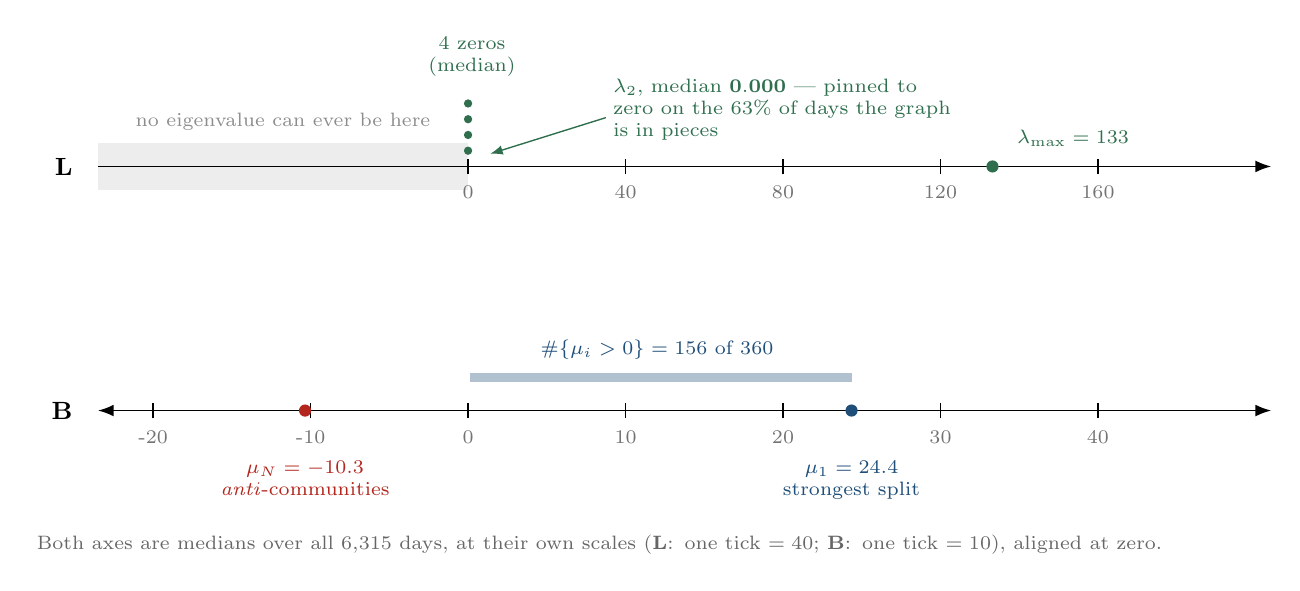
\begin{tikzpicture}[font=\small,x=1cm,y=1cm]

% ---------- Laplacian axis ----------
\begin{scope}[shift={(0,0)}]
  \fill[black!7] (-4.7,-0.30) rectangle (0,0.30);
  \node[font=\scriptsize,color=black!45,align=center,anchor=south] at (-2.35,0.34) {no eigenvalue can ever be here};
  \draw[-{Latex[length=2mm]},line width=.6pt] (-4.7,0) -- (10.2,0);
  \foreach \v in {0,40,80,120,160}{
    \pgfmathsetmacro\xx{\v/20}
    \draw[line width=.5pt] (\xx,-0.10) -- (\xx,0.10);
    \node[font=\scriptsize,color=black!55,anchor=north] at (\xx,-0.13) {\v};}
  \foreach \k in {0,1,2,3}{
    \pgfmathsetmacro\yy{0.20+0.20*\k}
    \fill[LapC] (0,\yy) circle (1.5pt);}
  \fill[LapC] (6.66,0) circle (2.2pt);
  \node[anchor=south,font=\scriptsize,color=LapC,align=center] at (0.05,1.02)
    {$4$ zeros\\(median)};
  \node[anchor=west,font=\scriptsize,color=LapC,align=left] at (6.85,0.36)
    {$\lambda_{\max}=133$};
  \draw[-{Latex[length=1.6mm]},LapC,line width=.5pt] (1.75,0.62) -- (0.28,0.16);
  \node[anchor=west,font=\scriptsize,color=LapC,align=left,text width=44mm] at (1.72,0.72)
    {$\lambda_2$, median $\mathbf{0.000}$ --- pinned to zero on the
     $63\%$ of days the graph is in pieces};
  \node[anchor=east,font=\small] at (-4.9,0) {$\Lap$};
\end{scope}

% ---------- modularity axis ----------
\begin{scope}[shift={(0,-3.1)}]
  \draw[{Latex[length=2mm]}-{Latex[length=2mm]},line width=.6pt] (-4.7,0) -- (10.2,0);
  \foreach \v in {-20,-10,0,10,20,30,40}{
    \pgfmathsetmacro\xx{\v/5}
    \draw[line width=.5pt] (\xx,-0.10) -- (\xx,0.10);
    \node[font=\scriptsize,color=black!55,anchor=north] at (\xx,-0.13) {\v};}
  \draw[ModC!35,line width=3pt] (0.02,0.42) -- (4.87,0.42);
  \node[anchor=south,font=\scriptsize,color=ModC,align=center] at (2.4,0.52)
    {$\#\{\mu_i>0\}=156$ of $360$};
  \fill[ScalC] (-2.07,0) circle (2.2pt);
  \fill[ModC]  (4.87,0) circle (2.2pt);
  \node[anchor=north,font=\scriptsize,color=ScalC,align=center] at (-2.07,-0.52)
    {$\mu_N=-10.3$\\\emph{anti}-communities};
  \node[anchor=north,font=\scriptsize,color=ModC,align=center] at (4.87,-0.52)
    {$\mu_1=24.4$\\strongest split};
  \node[anchor=east,font=\small] at (-4.9,0) {$\Bmat$};
\end{scope}

\node[font=\scriptsize,color=black!60,anchor=north west,text width=150mm] at (-5.6,-4.55)
  {Both axes are medians over all $6{,}315$ days, at their own scales
   ($\Lap$: one tick $=40$; $\Bmat$: one tick $=10$), aligned at zero.};
\end{tikzpicture}
\caption{The two spectra, drawn on the same networks. $\Lap$ is positive
semi-definite, so its entire left half is unreachable; the only thing it can
report about missing structure is how many pieces the graph has already fallen
into, and once it has fallen into pieces $\lambda_2$ is identically zero and
carries nothing. $\Bmat$ straddles zero, and its negative half is a live signal
about pairs of stocks that are avoiding each other.}
\label{fig:spectra}
\end{figure}

\begin{table}[h]
\centering\small
\caption{The three operators whose full spectrum the probe computes on each of
the $6{,}315$ daily networks. $\Cmat$ is included because it is what exists
\emph{before} thresholding --- the object the pipeline starts from.}
\label{tab:operators}
\begin{tabular}{@{}llp{78mm}@{}}
\toprule
& definition & what its spectrum reports \\
\midrule
$\Lap$ & $\mathbf{D}-\Amat$ & how well connected the network is, and where it
would break. The multiplicity of the zero eigenvalue is the number of
disconnected pieces \\[3pt]
$\Bmat$ & $\Amat-\dvec\dvec^{\!\top}\!/2m$ & community structure (positive end)
and anti-community structure (negative end) \\[3pt]
$\Cmat$ & the raw correlation matrix, \emph{before} thresholding & how much
everything is moving together; the leading eigenvalue is the market mode \\
\bottomrule
\end{tabular}
\end{table}

\section{One ruler for every candidate}
\label{sec:ruler}

Before any of these can be compared, they have to be put on a common scale.
This section is the scoring apparatus; it is Silva's replication's own, unchanged.

\textbf{Levels cannot be scored.} $\lambda_2$ drifts over 25 years; ``$\lambda_2
= 3.1$'' means nothing on its own. What matters is whether today is unusual
\emph{relative to recent normal}. So every series is converted to a trailing
250-day $z$-score,
\[
  z(t)=\frac{x(t)-\operatorname{mean}\big(x(t-250),\dots,x(t-1)\big)}
             {\operatorname{sd}\big(x(t-250),\dots,x(t-1)\big)},
\]
where $z=0$ means today is typical and $z=3$ means three standard deviations
from the last year's normal. The window uses \emph{only days strictly before
today}, which is what makes this an honest detector rather than a description.

\textbf{The crisis windows were fixed in advance.} Seventeen events --- Black
Monday, Friday the 13th, Black Wednesday, October 1997, Russia/LTCM, Boo.com,
9/11, China 2007, Dubai 2009, and eight diffuse regimes --- were written down in
Phase 0 of the replication, before any network existed, so no detector can have
been tuned to them. Nine are tagged \emph{sharp}, and those are what everything
below is scored against: $2.68\%$ of days, about $169$ of the $6{,}315$.

\textbf{Accuracy is useless at that base rate}, since a detector that says ``no
crisis'' every day is $97.3\%$ accurate and worthless. So the score is ROC-AUC:

\begin{aside}{What AUC means.}
Rank all $6{,}315$ days by the detector's $z$-score. Then
\textbf{AUC is the probability that a randomly chosen crisis day ranks above a
randomly chosen calm day.} $0.50$ is a coin flip and carries no information;
$1.00$ is perfect; $0.75$ means that picking one crisis day and one calm day at
random, three times in four the crisis day scores higher.
\end{aside}

\noindent Two things to declare about this ruler, both of which cut against the
numbers rather than for them.

\begin{enumerate}
\item \textbf{Each statistic was tried in both directions} --- ``crisis $=$
spike'' and ``crisis $=$ drop'' --- and the better score kept. That flatters
every entry in the table slightly, the new ones and the incumbents alike.
\item \textbf{$\lambda_2$'s detector is undefined on some days.} On the $63\%$
of days when the graph is disconnected $\lambda_2$ is exactly zero, and over
long stretches of those the trailing standard deviation is zero too, so the
$z$-score does not exist. This is a genuine property of the Fiedler value on
these graphs rather than a scoring artifact, and it is part of why it scores as
it does.
\end{enumerate}

The point of the apparatus is that \emph{every} statistic --- incumbent and new
--- goes through the identical detector. As a control, the probe re-derives the
replication's own stored scores for $\Q$ and $\tau$ and gets
$0.5380684370$ and $0.8071316467$, matching to ten decimal places. The new
numbers therefore sit on exactly the ruler the published ones do.

\section{Discrepancy in the scalar: the reduction loses the signal}
\label{sec:disc}

Silva's pipeline already built $6{,}315$ daily networks. The probe walks through
them and computes the full spectrum of $\Lap$, $\Bmat$ and $\Cmat$ for each
one --- three $360\times360$ eigendecompositions per day, about six minutes on
one core --- and scores every resulting statistic through the detector of
\S\ref{sec:ruler}. Figure~\ref{fig:leaderboard} and Table~\ref{tab:leaderboard}
are the result.

\begin{figure}[t]
\centering
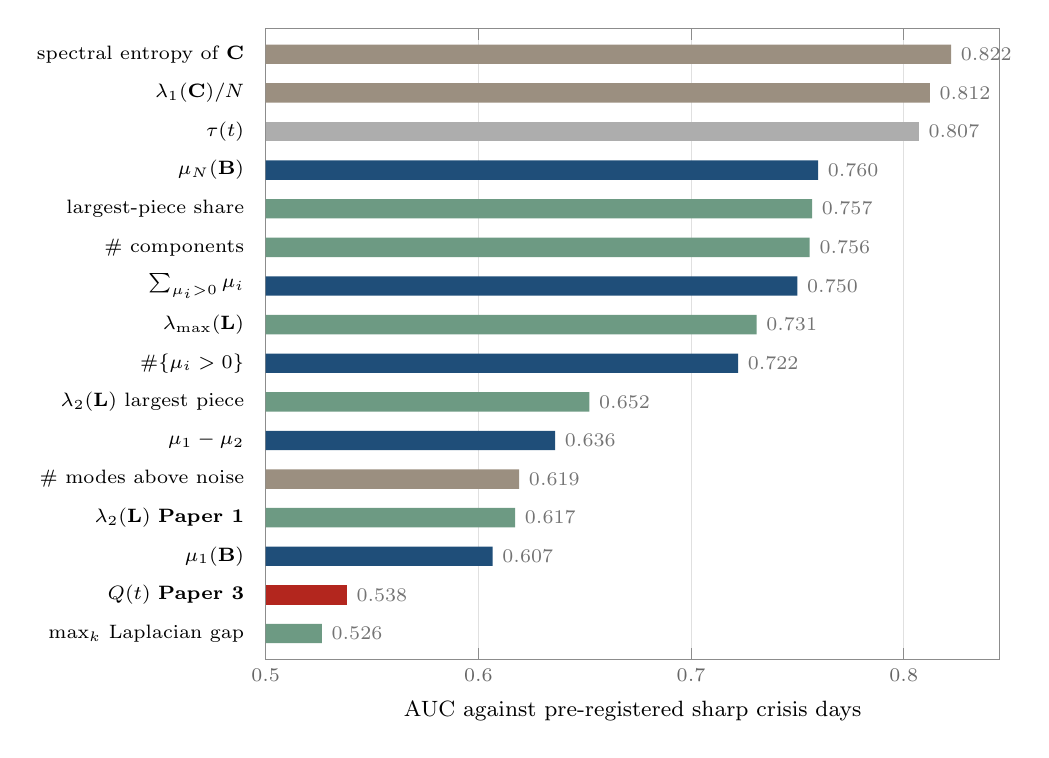
\begin{tikzpicture}
\begin{axis}[
  xbar, width=10.9cm, height=9.6cm,
  xmin=0.5, xmax=0.845,
  bar width=7pt, bar shift=0pt,
  enlarge y limits=0.045,
  axis line style={draw=black!45,line width=.4pt},
  tick style={draw=black!45}, ytick style={draw=none},
  xtick={0.5,0.6,0.7,0.8},
  xticklabel style={font=\scriptsize,color=black!60},
  xlabel={\footnotesize AUC against pre-registered sharp crisis days},
  xmajorgrids=true, grid style={draw=black!12,line width=.3pt},
  symbolic y coords={maxgap,qdyn,mu1,lam2,nmodes,gap12,lcclam2,npos,lmax,
                     tracepos,nzero,lccfrac,muN,tau,absr,entropy},
  ytick={maxgap,qdyn,mu1,lam2,nmodes,gap12,lcclam2,npos,lmax,
         tracepos,nzero,lccfrac,muN,tau,absr,entropy},
  yticklabels={%
    {$\max_k$ Laplacian gap},
    {$\Q(t)$\ \textbf{Paper 3}},
    {$\mu_1(\Bmat)$},
    {$\lambda_2(\Lap)$\ \textbf{Paper 1}},
    {\# modes above noise},
    {$\mu_1-\mu_2$},
    {$\lambda_2(\Lap)$ largest piece},
    {$\#\{\mu_i>0\}$},
    {$\lambda_{\max}(\Lap)$},
    {$\sum_{\mu_i>0}\mu_i$},
    {\# components},
    {largest-piece share},
    {$\mu_N(\Bmat)$},
    {$\tau(t)$},
    {$\lambda_1(\Cmat)/N$},
    {spectral entropy of $\Cmat$}},
  yticklabel style={font=\scriptsize},
  nodes near coords,
  nodes near coords style={font=\scriptsize,color=black!55,
      /pgf/number format/.cd,fixed,zerofill,precision=3}]

\addplot[draw=none,fill=CorrC!75] coordinates {
  (0.6192,nmodes) (0.8123,absr) (0.8223,entropy)};
\addplot[draw=none,fill=LapC!70] coordinates {
  (0.5264,maxgap) (0.6173,lam2) (0.6522,lcclam2)
  (0.7308,lmax) (0.7558,nzero) (0.7569,lccfrac)};
\addplot[draw=none,fill=ModC] coordinates {
  (0.6067,mu1) (0.6361,gap12) (0.7221,npos)
  (0.7500,tracepos) (0.7597,muN)};
\addplot[draw=none,fill=black!32] coordinates {(0.8071,tau)};
\addplot[draw=none,fill=ScalC] coordinates {(0.5381,qdyn)};
\end{axis}
\end{tikzpicture}
\\[1mm]
{\footnotesize
\textcolor{CorrC!70!black}{$\blacksquare$}~correlation matrix $\Cmat$ \quad
\textcolor{LapC}{$\blacksquare$}~Laplacian $\Lap$ \quad
\textcolor{ModC}{$\blacksquare$}~modularity matrix $\Bmat$ \quad
\textcolor{black!35}{$\blacksquare$}~construction \quad
\textcolor{ScalC}{$\blacksquare$}~the scalar $\Q$}
\caption{Every statistic, one ruler. Bars begin at $0.50$, so bar length is
information above a coin flip. $\Q(t)$ --- the quantity the paper is built on
--- is the shortest bar but one. Three readings of the matrix it is derived
from, in dark blue, reach $0.722$ to $0.760$.}
\label{fig:leaderboard}
\end{figure}

\begin{table}[t]
\centering\small
\caption{The same numbers with their definitions. ``Operator'' is which matrix
the statistic is read from. All are scored identically; $\Q$ and $\tau$ reproduce
the replication's stored values to ten decimal places.}
\label{tab:leaderboard}
\begin{tabular}{@{}lllr@{}}
\toprule
\textbf{Signal} & \textbf{Operator} & \textbf{What it measures} & \textbf{AUC} \\
\midrule
spectral entropy of $\Cmat$ & $\Cmat$ & how spread out the correlation structure is & 0.822 \\
$\lambda_1(\Cmat)/N$ & $\Cmat$ & share of variance in the top common factor & 0.812 \\
$\tau(t)$ & --- & the cut-off needed that day to keep $10\%$ of pairs & 0.807 \\
$\mu_N(\Bmat)$ & $\Bmat$ & $\star$\ strongest \emph{anti}-community & \textbf{0.760} \\
largest-piece share & $\Lap$ & fraction of stocks in the biggest component & 0.757 \\
\# components & $\Lap$ & zero eigenvalues of $\Lap$: how many pieces & 0.756 \\
$\sum_{\mu_i>0}\mu_i$ & $\Bmat$ & $\star$\ total community mass & \textbf{0.750} \\
$\lambda_{\max}(\Lap)$ & $\Lap$ & the densest node's local connectivity & 0.731 \\
$\#\{\mu_i>0\}$ & $\Bmat$ & $\star$\ community count, no algorithm & \textbf{0.722} \\
$\lambda_2(\Lap)$, largest piece & $\Lap$ & Fiedler value with fragmentation removed & 0.652 \\
$\mu_1-\mu_2$ & $\Bmat$ & modularity spectral gap & 0.636 \\
\# modes above the noise band & $\Cmat$ & how many groups are even resolvable & 0.619 \\
$\lambda_2(\Lap)$, whole graph & $\Lap$ & Fiedler value --- \textbf{Paper 1's indicator} & 0.617 \\
$\mu_1(\Bmat)$ & $\Bmat$ & leading modularity eigenvalue & 0.607 \\
$\Q(t)$ & partition & Louvain modularity --- \textbf{Paper 3's indicator} & \textbf{0.538} \\
$\max_k(\lambda_{k+1}-\lambda_k)$ & $\Lap$ & largest Laplacian gap (Kang et al.) & 0.526 \\
\bottomrule
\end{tabular}
\end{table}

\subsection{How to read \texorpdfstring{$\Q=0.538$}{Q = 0.538}}

Pick a random crash day and a random calm day. $\Q$ ranks the crash day higher
$53.8\%$ of the time. A coin manages $50\%$. Silva et al.\ build a 25-year
narrative on this quantity, and against the crises that narrative is about, it
is very nearly uninformative.

\textbf{And it came from a matrix that scores $0.760$.} The three starred rows
--- $\mu_N(\Bmat)$, $\sum_{\mu>0}\mu$, and $\#\{\mu>0\}$ --- are statistics of
the \emph{same matrix} $\Bmat$, on the \emph{same networks}, under the
\emph{same scoring}, and they reach $0.722$ to $0.760$. Nothing about the data
changed. The only thing that changed is that the matrix was read directly
instead of being pushed through Louvain and collapsed to a scalar.

That is the key discrepancy. Three details fill it in.

\textbf{The strongest modularity signal is the negative end.} $\mu_N$ ---
anti-communities, groups pulling apart --- beats every positive-side statistic
of $\Bmat$. That is precisely the thing thresholding is structurally incapable
of representing (Figure~\ref{fig:spectra}), and it is unexamined in finance.

\textbf{$\mu_1$ measures what Louvain is trying to measure, without the
instability.} In levels $\mu_1(\Bmat)$ correlates $0.761$ with $\Q$, so it is
largely tracking the same underlying quantity --- but deterministically. Louvain
is not: its seed-to-seed spread on a single day is $2.09\times$ the median
day-to-day move in $\Q$. Run it twice on identical data and the disagreement is
twice the size of the signal being studied. Even as a straight drop-in
replacement that is worth something.

\textbf{What this does \emph{not} say.} Paper 1's $\lambda_2$ scores $0.617$
here, and that is not a refutation of Paper 1. Cardoso \& Palomar learn a
regularised Laplacian on seven stocks; this is a thresholded 360-node
correlation network --- a different object entirely. The claim is narrower and
should stay narrow: \emph{on thresholded correlation networks of this kind}, the
Fiedler value is a weak detector. The same caution applies to Kang et al.'s
largest-gap statistic at $0.526$.

\section{Three mechanisms behind the empty scalar}
\label{sec:mech}

A discrepancy is worth more when its cause can be named. Three separate things
are going wrong at the Louvain step, and they are independent of one another.

\subsection{Louvain disagrees with itself}

Louvain is a greedy randomised search, so it returns a different partition on
every run. The replication measured how different. Normalised mutual information
between two seeds on the \emph{same day} is $0.543$; between consecutive days at
a \emph{fixed} seed it is $0.463$. In other words, two runs on identical data
agree only $0.079$ more than runs on genuinely different data. Expressed in the
units of the series itself, the seed-to-seed spread on one day is
$\mathbf{2.09\times}$ the median day-to-day move in $\Q$.

The consequence for a time series is direct: a meaningful fraction of the
day-to-day variation in $\Q(t)$ --- the variation the paper's 25-year narrative
is about --- is the random number generator.

\subsection{Louvain always finds communities, including in noise}

Louvain has no way to answer ``there is nothing here''. It always returns a
partition, and that partition always has a positive $\Q$. The replication ran
the control the paper did not: push i.i.d.\ Gaussian returns --- containing no
communities whatsoever --- through the entire pipeline unchanged.

\begin{aside}{The noise control.}
Pure noise gives $\Q = 0.2246\pm0.0067$, with a median of $7$ communities.\\
The real market gives $\Q = 0.2215\pm0.0413$.\\[2mm]
\emph{Structureless data comes out marginally more modular than the actual stock
market.}
\end{aside}

\noindent The mechanism is not mysterious. A correlation matrix is positive
semi-definite, so a high $\rho_{ij}$ and a high $\rho_{ik}$ force $\rho_{jk}$
up. Thresholding one therefore produces a graph that is \emph{transitive by
construction} --- full of triangles --- and transitive graphs are modular.
Measured on the noise networks, transitivity is $0.219$. A degree-preserving
null model cannot control for this, because rewiring destroys the geometry along
with the structure.

The right comparison is therefore each series against \emph{its own} null. The
market's $\Q=0.2215$ sits $+0.1150$ above its degree-sequence null of $0.1065$.
A second noise run, scored the same way, gives $\Q=0.2253$ against a null of
$0.1332$ --- an excess of $+0.0921$.\footnote{The two noise figures come from
different runs and are not interchangeable: $0.2246\pm0.0067$ is the
full-length Phase-3 level comparison quoted above, while $0.2253$ is the
101-day Phase-4 run that also carries its own matched null, which is what the
excess calculation needs. Both are recorded in
\texttt{results/phase4\_nulls.json} and \texttt{PITFALLS.md}.} So
\textbf{$80\%$ of the market's apparent excess modularity is reproduced by data
with no communities in it.}

\subsection{At this window length, there is very little to detect}

The previous subsection shows it happens. Random-matrix theory explains why it
must.

Each day, $64{,}620$ pairwise correlations are estimated from $30$ days of data
on $360$ stocks --- $10{,}800$ numbers. That is six times more output than
input, and it has an immediate arithmetic consequence: a correlation matrix
built from $30$ observations has \textbf{rank at most $29$}, so at least $331$
of its $360$ eigenvalues are exactly zero, forced by counting rather than by
anything about markets.

Marchenko--Pastur says how large the remaining ones get from estimation error
alone. With $N/\Delta t=360/30=12$, the noise band is
\[
  \big[(1-\sqrt{12})^2,\ (1+\sqrt{12})^2\big] \;=\; [\,6.07,\ 19.93\,].
\]
\textbf{Any eigenvalue below $19.93$ is indistinguishable from what pure noise
produces.} It is not evidence of structure. Counting, for each day, the
eigenvalues that escape above $19.93$ --- excluding the largest, which is the
market mode --- gives the right-hand panel of Figure~\ref{fig:mp}.

\begin{figure}[t]
\centering
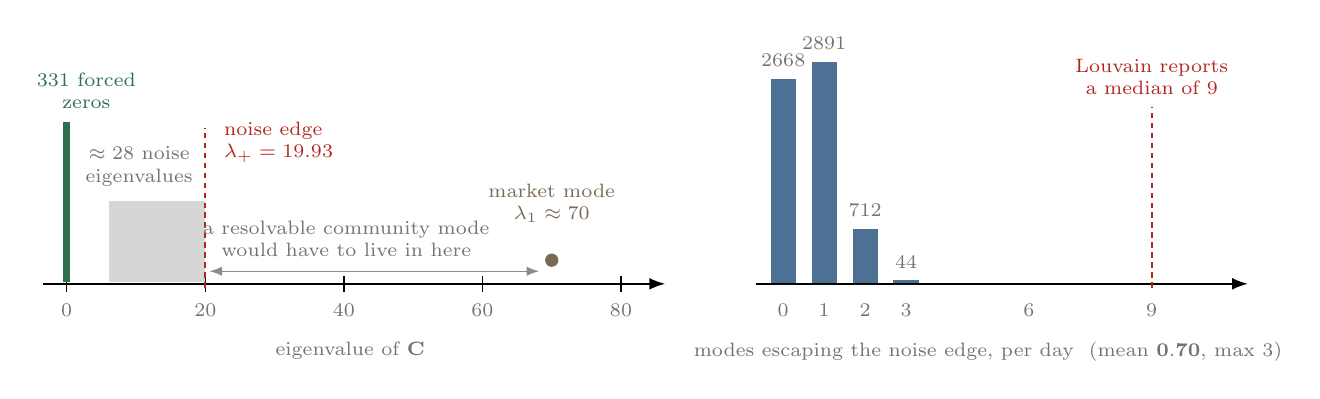
\begin{tikzpicture}[font=\small,x=1cm,y=1cm]

% ================= left: the spectrum of C on a typical day =================
\begin{scope}
  \def\sx{0.088}   % cm per eigenvalue unit
  \draw[-{Latex[length=2mm]},line width=.6pt] (-0.3,0) -- (7.6,0);
  \foreach \v in {0,20,40,60,80}{
    \draw[line width=.5pt] (\v*\sx,-0.10) -- (\v*\sx,0.10);
    \node[font=\scriptsize,color=black!55,anchor=north] at (\v*\sx,-0.13) {\v};}
  \node[font=\scriptsize,color=black!55,anchor=north] at (3.6,-0.62)
    {eigenvalue of $\Cmat$};

  % forced zeros
  \draw[LapC,line width=2.6pt] (0,0.02) -- (0,2.05);
  \node[font=\scriptsize,color=LapC,anchor=south,align=center] at (0.25,2.10)
    {$331$ forced\\zeros};

  % MP bulk
  \fill[black!16] (6.07*\sx,0.02) rectangle (19.93*\sx,1.05);
  \node[font=\scriptsize,color=black!55,anchor=south,align=center] at (0.92,1.12)
    {$\approx28$ noise\\eigenvalues};
  \draw[BadRed,line width=.9pt,dash pattern=on 2pt off 1.6pt]
    (19.93*\sx,-0.05) -- (19.93*\sx,1.98);
  \node[font=\scriptsize,color=BadRed,anchor=west,align=left,text width=30mm]
    at (19.93*\sx+0.12,1.80) {noise edge\\$\lambda_+=19.93$};

  % market mode
  \fill[CorrC] (70*\sx,0.30) circle (2.4pt);
  \node[font=\scriptsize,color=CorrC,anchor=south,align=center] at (70*\sx,0.66)
    {market mode\\$\lambda_1\approx70$};

  % the gap
  \draw[{Latex[length=1.6mm]}-{Latex[length=1.6mm]},black!45,line width=.5pt]
    (19.93*\sx+0.06,0.16) -- (70*\sx-0.16,0.16);
  \node[font=\scriptsize,color=black!55,anchor=south,align=center] at (3.55,0.22)
    {a resolvable community mode\\would have to live in here};
\end{scope}

% ================= right: how many actually do =================
\begin{scope}[shift={(9.1,0)}]
  \def\bx{0.52}   % cm per count unit
  \def\by{0.00098}% cm per day
  \draw[-{Latex[length=2mm]},line width=.6pt] (-0.35,0) -- (5.9,0);
  \foreach \v in {0,1,2,3}{
    \fill[ModC!80] (\v*\bx-0.16,0) rectangle (\v*\bx+0.16,{\by*0});
    \node[font=\scriptsize,color=black!55,anchor=north] at (\v*\bx,-0.13) {\v};}
  \foreach \v/\c in {0/2668,1/2891,2/712,3/44}{
    \fill[ModC!80] (\v*\bx-0.16,0.005) rectangle (\v*\bx+0.16,{\c*\by});
    \node[font=\scriptsize,color=black!55,anchor=south] at (\v*\bx,{\c*\by+0.03}) {\c};}
  \foreach \v in {6,9}{
    \node[font=\scriptsize,color=black!55,anchor=north] at (\v*\bx,-0.13) {\v};}
  \draw[ScalC,line width=.9pt,dash pattern=on 2pt off 1.6pt]
    (9*\bx,-0.05) -- (9*\bx,2.25);
  \node[font=\scriptsize,color=ScalC,anchor=south,align=center] at (9*\bx,2.28)
    {Louvain reports\\a median of $9$};
  \node[font=\scriptsize,color=black!55,anchor=north,align=center] at (2.6,-0.62)
    {modes escaping the noise edge, per day\ \ (mean $\mathbf{0.70}$, max $3$)};
\end{scope}
\end{tikzpicture}
\caption{\textbf{Left:} where the eigenvalues of one day's correlation matrix
actually sit. \textbf{Right:} how many of them clear the noise edge, counted
over all $6{,}315$ days, against the number of communities Louvain reports.
There is on average less than one statistically resolvable group per day beyond
the market itself, and none at all on $2{,}668$ days.}
\label{fig:mp}
\end{figure}

\noindent The result:

\begin{aside}{Detectable structure per day.}
Mean count $\mathbf{0.70}$. Maximum $3$. Exactly zero on $\mathbf{2{,}668}$ of
$6{,}315$ days.\\[1mm]
Louvain, on the same data, reports a \textbf{median of nine} communities every
day, and the paper narrates their 25-year dynamics.
\end{aside}

\noindent Most of those nine are not detectable structure; they are the
algorithm partitioning noise. And this does not indict Silva et al.\ alone ---
$\Delta t=30$ with a few hundred stocks is standard across this entire
literature.

\section{Discrepancy in the duality: two indicators that should be one number}
\label{sec:duality}

The prompt presupposes that comparing the Laplacian and the modularity matrix
is a meaningful thing to do. It is worth checking that presupposition, because
there is a theorem that appears to destroy it.

\textbf{The identity.} On a connected graph in which \emph{every} node has the
same degree $d$, it is exactly true that
\[
  \lambda_2(\Lap) \;+\; \mu_1(\Bmat) \;=\; d .
\]
Both operators are built on top of the same adjacency matrix, and on a regular
graph both reduce to reading the adjacency spectrum --- one from the bottom, one
from the top. \textbf{They are the same number, backwards.}

If that held on these networks, then ``compare Paper 1's indicator with Paper
3's'' would be a null question. There would be one indicator with two names, and
the study would be measuring nothing.

\textbf{Why it ought to nearly hold here.} Silva's fixed-density construction
pins the average degree at exactly $35.90$ every single day --- not
approximately, by construction (\S\ref{sec:pipeline}). These graphs are about as
close to regular as any real financial network one could build.

\textbf{What was measured.} Figure~\ref{fig:duality} and
Table~\ref{tab:duality}.
\begin{figure}[t]
\centering
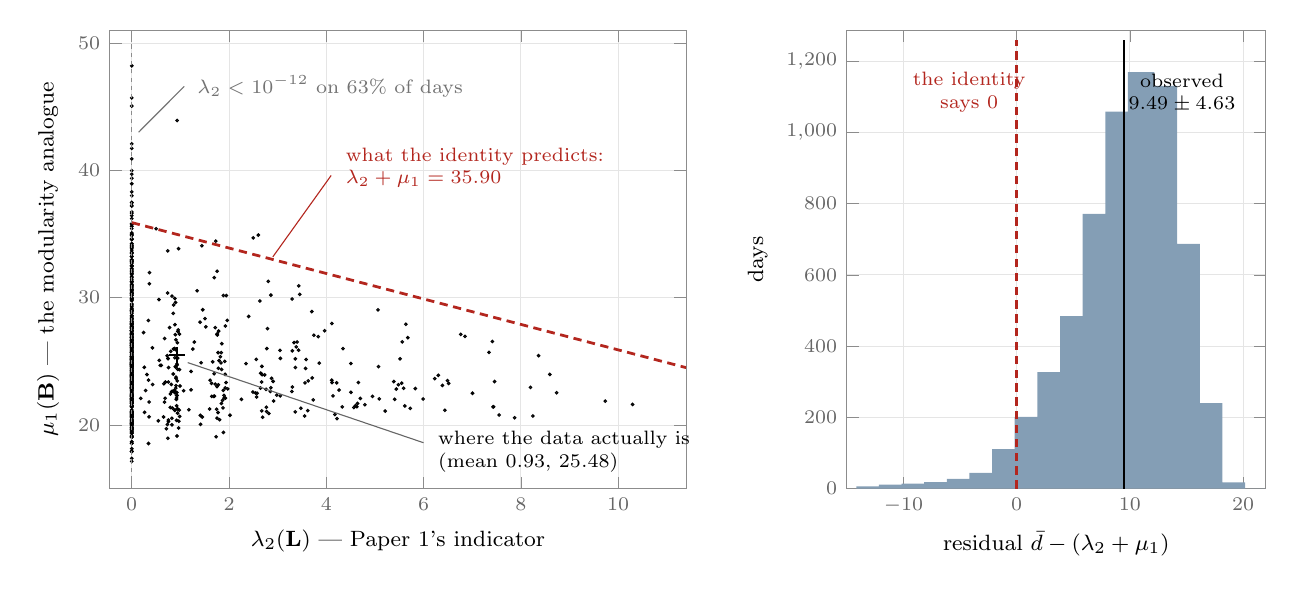
\begin{tikzpicture}
\begin{axis}[
  name=sc, width=8.9cm, height=7.4cm,
  xmin=-0.45, xmax=11.4, ymin=15, ymax=51,
  xlabel={\footnotesize $\lambda_2(\Lap)$ --- Paper 1's indicator},
  ylabel={\footnotesize $\mu_1(\Bmat)$ --- the modularity analogue},
  label style={font=\footnotesize},
  tick label style={font=\scriptsize,color=black!60},
  axis line style={draw=black!45,line width=.4pt},
  tick style={draw=black!45},
  grid=both, grid style={draw=black!10,line width=.3pt},
  clip mode=individual]

\addplot[only marks,mark=*,mark size=0.45pt,
         mark options={draw=none,fill=ModC,fill opacity=0.38}] coordinates {(0.000,25.05) (6.765,27.12) (7.415,26.56) (5.439,22.82) (3.429,25.87) (0.946,24.36) (0.000,24.72) (0.000,22.03) (0.000,19.69) (0.000,21.49) (0.000,20.31) (0.358,21.80) (1.067,22.69) (0.000,27.09) (0.000,25.38) (0.000,22.20) (0.000,22.66) (0.982,24.35) (1.256,25.96) (0.000,22.96) (0.000,21.72) (0.000,23.15) (2.349,24.82) (1.700,22.26) (3.362,21.02) (0.882,22.69) (1.219,22.76) (0.000,22.72) (0.000,27.38) (0.000,25.14) (0.000,26.32) (0.000,26.73) (0.746,25.22) (0.801,25.78) (2.491,22.58) (1.926,22.11) (0.000,24.30) (0.000,24.90) (0.000,25.55) (0.000,25.57) (0.000,26.55) (0.000,23.65) (0.000,22.05) (0.000,22.37) (4.263,22.74) (4.628,21.43) (3.620,21.12) (4.506,24.82) (1.693,24.02) (0.000,21.01) (0.000,26.47) (0.000,29.05) (0.000,29.93) (0.000,19.33) (0.000,41.73) (0.000,42.08) (0.000,40.90) (0.000,30.33) (0.000,21.72) (0.000,22.31) (0.000,17.37) (0.000,18.67) (0.000,21.47) (0.000,22.65) (0.000,19.64) (1.450,20.62) (0.830,22.65) (0.000,24.24) (0.000,23.33) (0.000,20.24) (0.000,22.07) (0.000,19.46) (0.000,19.37) (0.000,22.24) (0.000,19.98) (0.000,19.04) (0.000,17.91) (0.344,18.54) (0.000,17.90) (0.000,19.76) (0.000,19.16) (0.000,18.56) (0.000,19.34) (0.742,18.95) (0.967,20.29) (0.655,20.63) (0.000,20.71) (0.000,20.05) (0.547,20.32) (0.000,18.56) (0.000,19.60) (3.302,25.82) (2.681,23.95) (3.364,25.19) (2.653,24.06) (2.761,22.80) (0.711,19.70) (0.000,21.65) (0.000,21.43) (0.000,19.60) (0.000,20.76) (0.000,19.81) (2.820,20.90) (0.754,20.39) (2.020,20.76) (0.923,22.32) (0.888,21.18) (0.000,22.20) (0.924,21.50) (0.941,20.92) (1.877,21.34) (3.302,22.98) (0.825,20.52) (1.646,22.24) (0.000,22.43) (0.660,23.23) (0.000,28.02) (0.000,27.89) (0.000,27.57) (0.000,26.11) (0.263,20.99) (1.175,21.19) (1.686,22.25) (0.693,23.37) (0.345,23.52) (0.000,26.07) (0.000,27.58) (0.000,26.65) (0.000,27.43) (1.851,26.38) (0.928,24.78) (0.756,24.51) (0.965,19.76) (0.922,20.36) (0.355,20.64) (0.755,20.25) (0.985,20.67) (0.885,21.14) (0.906,22.89) (0.882,22.54) (0.000,20.81) (1.780,23.15) (0.000,19.03) (0.000,24.20) (0.000,22.26) (0.000,23.89) (0.000,25.22) (0.000,22.70) (0.000,20.15) (0.000,19.09) (0.000,21.45) (0.000,22.91) (0.000,25.41) (0.000,24.25) (1.920,23.97) (0.000,23.54) (0.000,20.38) (0.000,22.81) (0.000,21.01) (0.000,19.84) (0.932,22.31) (0.686,22.09) (0.000,22.00) (0.909,23.09) (0.838,21.32) (1.602,21.25) (0.000,21.51) (1.427,24.89) (0.000,26.85) (0.981,27.14) (0.000,25.70) (0.313,23.96) (1.414,20.05) (2.255,22.01) (2.919,21.88) (0.000,20.11) (0.000,20.10) (0.000,19.10) (0.930,19.13) (2.579,22.49) (4.220,20.49) (1.807,20.41) (0.733,20.03) (0.794,22.43) (0.921,22.11) (0.674,21.79) (0.910,23.75) (1.795,25.06) (1.786,27.37) (3.587,25.14) (1.963,28.22) (2.773,21.05) (1.897,22.10) (4.507,22.56) (4.214,23.31) (0.000,20.58) (0.000,20.79) (0.000,20.69) (1.775,20.97) (5.388,23.41) (2.648,22.90) (2.676,24.60) (3.056,25.23) (1.847,24.36) (1.754,23.01) (1.939,23.33) (3.554,20.70) (2.673,21.11) (1.641,23.27) (1.912,24.99) (2.561,25.15) (1.835,24.88) (0.915,22.00) (2.567,22.19) (4.566,21.37) (7.874,20.56) (8.247,20.70) (4.602,21.51) (6.493,23.48) (6.389,23.10) (6.303,23.90) (6.231,23.64) (1.523,27.71) (0.677,26.79) (0.861,29.42) (0.737,30.37) (0.881,26.01) (0.937,23.46) (2.982,22.34) (2.671,23.37) (4.700,22.08) (3.628,23.46) (3.574,24.44) (2.875,23.66) (4.177,20.82) (9.738,21.87) (7.429,21.41) (6.438,21.15) (8.198,22.95) (7.007,22.49) (5.551,23.28) (3.711,23.69) (8.597,23.97) (5.676,26.85) (8.365,25.44) (5.518,25.19) (3.400,26.52) (3.966,27.40) (1.924,22.91) (3.479,21.31) (5.590,22.88) (8.737,22.53) (6.853,26.96) (3.382,26.13) (1.776,25.68) (0.897,24.58) (2.861,22.92) (0.000,24.14) (0.000,22.45) (0.000,26.08) (0.000,26.66) (1.505,28.35) (2.635,29.74) (2.769,21.39) (1.974,22.83) (0.927,22.55) (0.827,20.01) (0.792,21.37) (5.992,22.04) (4.950,22.24) (5.830,22.86) (4.119,23.33) (1.754,20.53) (1.885,19.41) (0.000,20.14) (0.000,19.83) (1.733,19.07) (2.691,20.61) (0.955,27.47) (2.777,26.00) (0.872,22.71) (1.610,23.51) (4.112,23.51) (7.348,25.70) (5.636,27.91) (5.074,24.58) (0.752,23.37) (0.000,22.01) (0.976,21.17) (1.883,22.72) (6.517,23.26) (10.299,21.61) (5.090,22.05) (5.212,21.09) (4.661,23.33) (2.791,27.57) (0.939,26.46) (1.945,30.16) (0.000,28.58) (0.000,26.41) (0.000,23.45) (0.941,21.27) (4.794,21.59) (7.442,21.43) (7.556,20.78) (4.644,21.69) (5.615,21.49) (4.138,22.28) (3.563,23.30) (3.745,27.05) (3.835,26.94) (7.460,23.41) (2.852,22.63) (0.932,24.70) (3.048,25.86) (1.780,24.45) (1.897,22.32) (0.853,24.00) (0.895,22.53) (0.000,20.20) (0.000,23.02) (0.000,22.11) (1.411,20.75) (1.745,21.23) (0.429,23.17) (4.344,25.99) (1.759,27.07) (3.702,28.91) (3.298,29.89) (1.460,29.05) (0.000,29.84) (0.000,27.54) (0.000,29.38) (0.000,28.34) (0.000,23.14) (1.843,21.69) (3.731,21.97) (3.053,22.28) (4.329,21.42) (5.406,22.01) (5.482,23.16) (5.727,21.30) (3.855,24.86) (0.907,24.54) (0.000,26.89) (0.000,26.80) (1.287,26.51) (1.925,27.77) (2.548,22.50) (3.292,22.63) (1.867,21.93) (2.733,23.93) (0.992,23.06) (0.000,23.50) (0.000,23.58) (0.000,24.60) (0.000,24.94) (0.242,27.26) (0.000,24.46) (0.816,22.59) (0.745,25.21) (0.565,25.07) (0.000,24.68) (0.586,24.68) (0.185,22.08) (0.000,20.88) (0.000,21.03) (0.000,20.46) (0.000,19.50) (0.000,20.46) (0.000,18.69) (0.000,21.02) (0.000,23.07) (0.000,25.70) (0.000,20.29) (0.000,22.34) (0.000,25.10) (0.000,20.96) (0.000,21.51) (0.000,21.95) (0.728,25.44) (0.000,20.32) (0.000,24.65) (0.000,22.85) (0.000,22.89) (2.907,23.42) (0.000,23.94) (0.000,24.59) (0.000,24.74) (0.000,25.08) (0.000,24.48) (0.000,24.32) (0.607,24.68) (0.000,22.10) (0.000,23.08) (0.000,26.66) (0.000,25.24) (0.000,25.39) (0.000,24.76) (0.000,22.55) (0.000,23.22) (0.000,24.43) (0.000,24.24) (0.000,26.14) (0.777,27.65) (0.285,22.70) (0.912,23.66) (1.728,34.44) (1.884,30.17) (0.900,29.62) (0.886,29.94) (1.665,24.96) (0.909,26.69) (1.753,27.12) (0.887,27.88) (0.948,27.35) (0.501,35.42) (0.000,35.81) (0.000,34.08) (1.442,34.08) (2.861,30.20) (1.404,28.07) (0.901,25.92) (1.696,31.58) (2.497,34.70) (2.602,34.92) (0.963,33.85) (1.823,25.36) (0.856,25.96) (1.717,23.20) (0.813,23.18) (0.887,25.28) (0.342,28.21) (0.000,28.33) (0.000,25.70) (1.841,25.68) (1.758,27.16) (5.562,26.53) (3.365,24.51) (0.000,26.62) (0.000,26.36) (0.257,24.53) (1.219,24.20) (3.338,26.47) (0.000,27.75) (0.000,20.46) (0.000,20.61) (0.000,23.36) (0.000,23.60) (0.361,31.09) (0.000,32.51) (0.000,27.70) (1.343,30.54) (1.756,32.08) (3.434,30.92) (0.000,30.52) (0.000,28.14) (0.000,26.68) (1.717,27.65) (4.114,27.97) (5.064,29.04) (2.405,28.52) (3.454,30.26) (2.808,31.28) (0.853,28.76) (0.000,26.59) (0.895,27.09) (0.945,25.25) (0.000,25.28) (0.000,25.82) (0.425,26.06) (0.000,45.70) (0.000,45.06) (0.000,48.22) (0.933,43.92) (0.829,30.12) (0.000,28.15) (0.000,28.16) (0.000,25.45) (0.000,30.69) (0.000,30.33) (0.000,34.25) (0.000,39.71) (0.000,32.04) (0.000,33.54) (0.000,30.90) (0.740,33.68) (0.000,31.58) (0.000,31.30) (0.000,32.85) (0.000,33.95) (0.000,24.73) (0.000,19.41) (0.000,22.28) (0.000,22.05) (0.000,21.18) (0.000,24.88) (0.000,24.85) (0.000,31.16) (0.000,30.37) (0.000,31.91) (0.000,32.50) (0.000,30.55) (0.000,27.38) (0.000,27.42) (0.000,29.00) (0.000,31.56) (0.000,27.18) (0.000,33.22) (0.000,32.98) (0.000,27.65) (0.000,27.08) (0.000,23.53) (0.000,23.91) (0.000,23.88) (0.000,23.97) (0.000,26.43) (0.000,24.08) (0.000,23.79) (0.000,27.70) (0.000,25.30) (0.000,26.11) (0.000,25.36) (0.000,24.80) (0.000,26.24) (0.000,24.81) (0.000,23.29) (0.000,23.67) (0.000,22.83) (0.000,20.68) (0.000,21.06) (0.000,21.04) (0.000,22.05) (0.000,21.78) (0.000,20.02) (0.000,24.65) (0.000,25.34) (0.000,21.70) (0.000,24.11) (0.000,21.93) (0.000,17.14) (0.000,20.22) (0.000,17.93) (0.000,19.78) (0.000,21.40) (0.000,18.13) (0.000,20.86) (0.000,22.32) (0.000,24.07) (0.000,20.14) (0.000,26.87) (0.000,26.24) (0.000,25.71) (0.000,25.11) (0.000,32.29) (0.000,27.64) (0.000,23.39) (0.000,20.06) (0.000,21.11) (0.000,19.72) (0.000,22.29) (0.000,20.88) (0.000,21.47) (0.000,21.82) (0.000,23.79) (0.000,29.02) (0.559,29.85) (0.365,31.97) (0.000,27.15) (0.000,27.98) (0.000,26.61) (0.000,22.13) (0.000,22.10) (0.000,23.76) (0.000,27.00) (0.000,29.48) (0.000,26.69) (0.000,23.45) (0.000,23.19) (0.000,23.46) (0.000,28.53) (0.000,26.01) (0.000,27.45) (0.000,24.84) (0.000,23.75) (0.000,21.89) (0.000,20.79) (0.000,22.86) (0.000,23.84) (0.000,28.95) (0.000,28.10) (0.000,31.88) (0.000,32.70) (0.000,33.24) (0.000,34.58) (0.000,34.63) (0.000,32.96) (0.000,27.71) (0.000,25.93) (0.000,24.58) (0.000,27.39) (0.000,25.02) (0.000,27.67) (0.000,30.17) (0.000,28.90) (0.000,28.34) (0.000,27.95) (0.000,26.21) (0.000,27.17) (0.000,27.55) (0.000,24.26) (0.000,19.94) (0.000,22.26) (0.000,32.19) (0.000,31.67) (0.000,30.62) (0.000,34.57) (0.000,30.98) (0.000,25.73) (0.000,23.75) (0.000,31.42) (0.000,39.38) (0.000,34.88) (0.000,36.44) (0.000,32.02) (0.000,25.36) (0.000,24.99) (0.000,27.99) (0.000,26.37) (0.000,27.17) (0.000,28.16) (0.000,28.30) (0.000,27.11) (0.000,27.70) (0.000,26.86) (0.000,29.16) (0.000,28.43) (0.000,31.03) (0.000,30.65) (0.000,35.80) (0.000,38.01) (0.000,35.62) (0.000,34.95) (0.000,30.02) (0.000,26.94) (0.000,23.91) (0.000,23.41) (0.000,21.82) (0.000,21.01) (0.000,23.71) (0.000,24.93) (0.000,33.47) (0.000,35.08) (0.000,32.90) (0.000,32.13) (0.000,30.53) (0.000,22.96) (0.000,21.01) (0.000,22.97) (0.000,24.85) (0.000,30.32) (0.000,32.00) (0.000,31.29) (0.000,30.78) (0.000,23.11) (0.000,23.94) (0.000,24.39) (0.000,29.30) (0.000,27.86) (0.000,27.78) (0.000,20.29) (0.000,24.83) (0.000,27.12) (0.000,25.80) (0.000,24.44) (0.000,26.04) (0.000,28.04) (0.000,27.06) (0.000,38.95) (0.000,37.46) (0.000,37.48) (0.000,37.19) (0.000,25.84) (0.000,24.74) (0.000,22.90) (0.000,25.90) (0.000,36.21) (0.000,36.62) (0.000,35.42) (0.000,37.25) (0.000,28.60) (0.000,30.34) (0.000,32.77) (0.000,33.73) (0.000,34.14) (0.000,35.77) (0.000,31.81) (0.000,39.98) (0.000,38.31) (0.000,36.73) (0.000,32.82) (0.000,25.41) (0.000,25.65) (0.000,25.39) (0.000,27.40) (0.000,30.93) (0.000,35.00) (0.000,29.90) (0.000,25.26) (0.000,22.26) (0.000,23.17) (0.000,22.40) (0.000,30.22) (0.000,33.97) (0.000,35.60) (0.000,32.85) (0.000,30.61) (0.000,33.57) (0.000,34.03) (0.000,27.40) (0.000,29.85) (0.000,29.79) (0.000,31.25) (0.000,30.90) (0.000,26.45) (0.000,28.77) (0.000,26.15) (0.000,27.18) (0.000,29.94) (0.000,28.99) (0.000,30.21) (0.000,33.24) (0.000,32.53) (0.000,25.41) (0.000,29.51) (0.000,32.45) (0.000,34.25) (0.000,33.25) (0.000,34.92) (0.000,33.85) (0.000,29.75) (0.000,26.47) (0.000,26.39) (0.000,26.84) (0.000,24.51) (0.000,24.00) (0.000,22.87) (0.000,23.80) (0.000,23.99) (0.000,22.89) (0.000,22.91) (0.000,26.26) (0.000,27.63) (0.000,26.42) (0.000,29.96) (0.000,30.39) (0.000,26.94) (0.000,23.18) (0.000,20.66) (0.000,21.99) (0.000,24.92) (0.000,23.26) (0.000,27.27) (0.000,29.18) (0.000,24.23) (0.000,22.79) (0.000,25.14) (0.000,24.74) (0.000,28.80) (0.000,27.87) (0.000,27.11) (0.000,31.00) (0.000,26.63) (0.000,24.73) (0.000,23.90) (0.000,23.91) (0.000,24.94) (0.000,23.78) (0.000,20.38) (0.000,20.09) (0.000,20.55) (0.000,22.92) (0.000,22.93) (0.000,21.43) (0.000,24.33) (0.000,25.80) (0.000,25.18) (0.000,23.34) (0.000,21.74) (0.000,21.66)};

\addplot[BadRed,line width=1pt,dash pattern=on 3pt off 2pt]
  coordinates {(0,35.90) (11.4,24.50)};
\node[font=\scriptsize,color=BadRed,anchor=west,align=left] at (axis cs:4.2,40.2)
  {what the identity predicts:\\$\lambda_2+\mu_1=35.90$};
\draw[BadRed,line width=.4pt] (axis cs:4.1,39.6) -- (axis cs:2.9,33.2);

\addplot[only marks,mark=+,mark size=3pt,line width=.9pt,black]
  coordinates {(0.931,25.481)};
\node[font=\scriptsize,anchor=west,align=left] at (axis cs:6.1,17.9)
  {where the data actually is\\(mean $0.93$, $25.48$)};
\draw[black!60,line width=.4pt] (axis cs:6.0,18.6) -- (axis cs:1.15,24.9);

\draw[black!45,line width=.4pt,dash pattern=on 1.5pt off 1.5pt]
  (axis cs:0,15) -- (axis cs:0,51);
\node[font=\scriptsize,color=black!55,anchor=west,align=left] at (axis cs:1.15,46.6)
  {$\lambda_2<10^{-12}$ on $63\%$ of days};
\draw[black!55,line width=.4pt] (axis cs:1.08,46.6) -- (axis cs:0.14,43.0);
\end{axis}

\begin{axis}[
  at={(sc.right of south east)}, anchor=left of south west, xshift=5mm,
  width=6.9cm, height=7.4cm,
  ymin=0, xmin=-15, xmax=22,
  xlabel={\footnotesize residual $\bar d-(\lambda_2+\mu_1)$},
  ylabel={\footnotesize days},
  label style={font=\footnotesize},
  tick label style={font=\scriptsize,color=black!60},
  axis line style={draw=black!45,line width=.4pt},
  tick style={draw=black!45}, xtick={-10,0,10,20},
  grid=both, grid style={draw=black!10,line width=.3pt}]

\addplot[ybar,bar width=9.6pt,draw=none,fill=ModC!55]
  coordinates {(-13,6) (-11,11) (-9,14) (-7,18) (-5,27) (-3,44) (-1,111) (1,201) (3,327) (5,484) (7,771) (9,1058) (11,1169) (13,1130) (15,687) (17,240) (19,17) (21,0)};
\draw[BadRed,line width=1pt,dash pattern=on 3pt off 2pt]
  (axis cs:0,0) -- (axis cs:0,1260);
\node[font=\scriptsize,color=BadRed,anchor=south,align=center]
  at (axis cs:-4.2,1030) {the identity\\says $0$};
\draw[black,line width=1pt] (axis cs:9.489,0) -- (axis cs:9.489,1260);
\node[font=\scriptsize,anchor=south,align=center]
  at (axis cs:14.6,1030) {observed\\$9.49\pm4.63$};
\end{axis}
\end{tikzpicture}
\caption{\textbf{Left:} the two indicators, one point per eight days. If the
identity held, every point would sit on the red line. \textbf{Right:} the
distribution of the shortfall. It is centred on $9.49$, not zero, and it is
\emph{wide} --- so it is not a fixed offset that could be subtracted away. The
vertical stripe at $\lambda_2\approx0$ is the fragmentation problem in one glance: on
$63\%$ of days the graph is already in pieces, the Fiedler value is identically
zero, and it cannot vary with $\mu_1$ at all.}
\label{fig:duality}
\end{figure}
\begin{table}[h]
\centering\small
\caption{The identity, tested three ways. The last two rows remove the two
obvious confounds --- days when the graph is in pieces, and the pieces
themselves --- and neither rescues it.}
\label{tab:duality}
\begin{tabular}{@{}lrl@{}}
\toprule
quantity & value & what it should be \\
\midrule
average degree $\bar d$ & $35.900$ & exact, every day, by construction \\
observed $\lambda_2+\mu_1$ & $26.411$ & $35.900$ \\
\midrule
residual $\bar d-(\lambda_2+\mu_1)$, all days & $\mathbf{9.489\pm4.627}$ & $0$ \\
\quad restricted to the $2{,}342$ one-piece days & $9.210\pm3.595$ & $0$ \\
\quad on the largest component only & $11.109\pm5.314$ & $0$ \\
\midrule
$\operatorname{corr}(\lambda_2,\mu_1)$, all days & $\mathbf{-0.187}$ & $-1$ \\
\quad one-piece days & $-0.119$ & $-1$ \\
\quad largest component & $-0.169$ & $-1$ \\
\bottomrule
\end{tabular}
\end{table}

Read the residual first. $\lambda_2+\mu_1$ should equal $35.90$ and instead
comes out at $26.41$: \textbf{the identity misses by $26\%$ of the mean degree.}
And the $\pm4.63$ matters as much as the $9.49$ --- the gap is not a fixed
offset one could subtract away, it moves by a third of its own size from day to
day. It is a live quantity.

The correlation is the cleaner statement. If $\lambda_2+\mu_1=\bar d$ with
$\bar d$ fixed, then whenever $\lambda_2$ rises $\mu_1$ must fall by exactly as
much: they would be perfectly anti-correlated, $r=-1$. Two variables with no
relationship at all give $r=0$. Observed: $\mathbf{r=-0.187}$. That is far
closer to unrelated than to identical.

\begin{aside}{Dual in theory, unrelated in practice.}
The two indicators the field has been using are \emph{provably the same number}
in the idealised case and \emph{empirically almost independent} on real market
networks.
\end{aside}

\noindent This is why the discrepancy is worth something rather than merely
being a defect. It rescues the comparison question. It stops being the weak
``which indicator wins?'' and becomes a sharp one:

\begin{quote}
\textbf{What is that $9.49$ made of, and does it carry market-stress
information?}
\end{quote}

There are three candidate constituents, and they are separable:

\begin{enumerate}
\item \textbf{Degree heterogeneity.} The identity assumes every node has degree
$d$. Only the \emph{average} is pinned at $35.90$; in reality some stocks have
five edges and some have a hundred and fifty.
\item \textbf{Fragmentation.} The graph breaks into disconnected pieces on
$63\%$ of days (and on $99.3\%$ of days after 2002). Whenever it does,
$\lambda_2$ is identically zero --- it cannot vary with anything. That is the
vertical stripe in Figure~\ref{fig:duality}, and it is also why restricting to
the largest component makes the residual \emph{worse}, not better.
\item \textbf{The market mode.} The common factor that dominates $\Cmat$
(\S\ref{sec:caveats}) enters both operators, but not symmetrically.
\end{enumerate}

Establishing which of the three carries the stress information is a structural
result about what the field's two incumbent indicators actually measure. It does
not depend on winning a horse race. That is direction D1.

\section{What weakens all of this}
\label{sec:caveats}

Three things cut against the results above. They are put here rather than in a
footnote because they are the first things a referee will raise, and because the
third one is currently unresolved.

\subsection{The strongest detectors are one signal, and it was found in 1999}

On any given day the single biggest pattern in stock returns is that everything
moves together. In $\Cmat$ this shows up as one dominant eigenvalue $\lambda_1$,
vastly larger than the rest; in a crash, correlations go towards one across the
board and $\lambda_1$ balloons. That is the mechanism behind ``diversification
fails exactly when you need it''.

This is old, established finance. $\lambda_1(\Cmat)/N$ is precisely the
\textbf{absorption ratio} of Kritzman et al.\ (2011), and its random-matrix
precursors are Laloux et al.\ and Plerou et al., 1999.

Now look again at the top of Figure~\ref{fig:leaderboard}: spectral entropy
$0.822$, absorption ratio $0.812$, $\tau(t)$ $0.807$. Those three are
\textbf{pairwise correlated above $0.99$ in levels}. A correlation of $0.99$
means they are the same series with different labels. And the component count
($0.756$) correlates $0.92$ with $\tau$, so really it is four.

\begin{aside}{The top of the table is not four discoveries.}
It is one discovery, and it was made in 1999.
\end{aside}

\subsection{Out of sample, nothing yet beats that baseline}

The real question is therefore whether the modularity spectrum adds anything
\emph{on top of} the market mode. Testing that honestly means fitting on one
period and evaluating on data never seen: fit before 2002, evaluate after
(Table~\ref{tab:oos}, Figure~\ref{fig:oos}).

\begin{table}[h]
\centering\small
\caption{Logistic detector, fitted on pre-2002 and evaluated on post-2002 (27
crisis days in the test period). Every addition helps in-sample and hurts out of
sample.}
\label{tab:oos}
\begin{tabular}{@{}lrr@{}}
\toprule
model & in-sample & out-of-sample \\
\midrule
market mode alone & $0.812$ & $\mathbf{0.730}$ \\
\quad $+\ \mu_1(\Bmat)$ & $0.822$ & $0.629$ \\
\quad $+\ \mu_N(\Bmat)$ & $0.810$ & $0.719$ \\
\quad $+\ \Q(t)$ & $0.831$ & $0.699$ \\
\quad $+\ \lambda_2(\Lap)$ on the largest component & $0.810$ & $0.700$ \\
\midrule
market mode $+$ the whole modularity spectrum & $0.823$ & $0.640$ \\
modularity spectrum alone & $0.806$ & $0.685$ \\
$\Q(t)$ alone & $0.538$ & $0.667$ \\
\bottomrule
\end{tabular}
\end{table}

\begin{figure}[t]
\centering
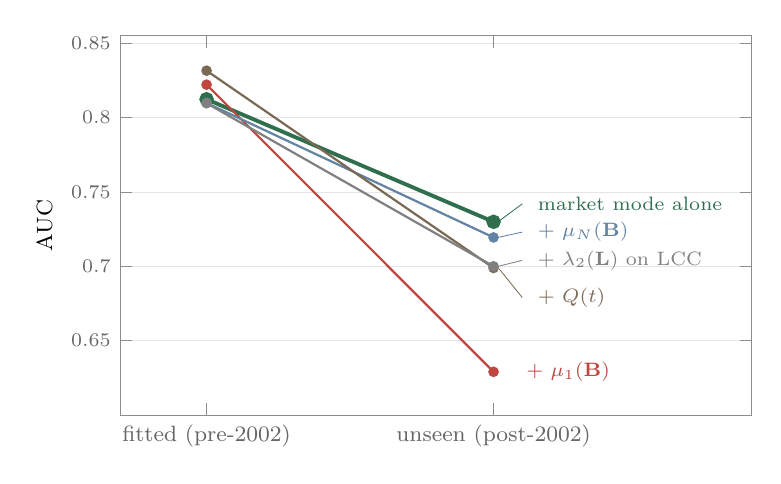
\begin{tikzpicture}
\begin{axis}[
  width=9.6cm, height=6.4cm,
  xmin=-0.30, xmax=1.90, ymin=0.60, ymax=0.855,
  xtick={0,1}, xticklabels={{\footnotesize fitted (pre-2002)},{\footnotesize unseen (post-2002)}},
  ytick={0.65,0.70,0.75,0.80,0.85},
  tick label style={font=\scriptsize,color=black!60},
  ylabel={\footnotesize AUC}, label style={font=\footnotesize},
  axis line style={draw=black!45,line width=.4pt}, tick style={draw=black!45},
  ymajorgrids=true, grid style={draw=black!10,line width=.3pt},
  clip mode=individual]

\addplot[LapC,line width=1.4pt,mark=*,mark size=1.9pt] coordinates {(0,0.8123)(1,0.7299)};
\node[font=\scriptsize,color=LapC,anchor=west] at (axis cs:1.12,0.7420) {market mode alone};
\draw[LapC,line width=.3pt] (axis cs:1.10,0.7420) -- (axis cs:1.02,0.7305);

\addplot[ScalC!85,line width=.8pt,mark=*,mark size=1.5pt] coordinates {(0,0.8221)(1,0.6291)};
\node[font=\scriptsize,color=ScalC!85,anchor=west] at (axis cs:1.08,0.6291) {$+\ \mu_1(\Bmat)$};

\addplot[ModC!70,line width=.8pt,mark=*,mark size=1.5pt] coordinates {(0,0.8098)(1,0.7194)};
\node[font=\scriptsize,color=ModC!70,anchor=west] at (axis cs:1.12,0.7230) {$+\ \mu_N(\Bmat)$};
\draw[ModC!70,line width=.3pt] (axis cs:1.10,0.7230) -- (axis cs:1.02,0.7196);

\addplot[CorrC,line width=.8pt,mark=*,mark size=1.5pt] coordinates {(0,0.8315)(1,0.6989)};
\node[font=\scriptsize,color=CorrC,anchor=west] at (axis cs:1.12,0.6790) {$+\ \Q(t)$};
\draw[CorrC,line width=.3pt] (axis cs:1.10,0.6790) -- (axis cs:1.02,0.6982);

\addplot[black!50,line width=.8pt,mark=*,mark size=1.5pt] coordinates {(0,0.8096)(1,0.7000)};
\node[font=\scriptsize,color=black!50,anchor=west] at (axis cs:1.12,0.7040) {$+\ \lambda_2(\Lap)$ on LCC};
\draw[black!50,line width=.3pt] (axis cs:1.10,0.7040) -- (axis cs:1.02,0.7002);
\end{axis}
\end{tikzpicture}
\caption{The same table as slopes. Every line falls, which is expected --- but
the plain market mode falls least and finishes highest, and adding $\mu_1$
produces both the largest in-sample gain and the largest out-of-sample loss.
That combination is the textbook fingerprint of overfitting: the extra variable
is not learning a market mechanism, it is memorising 1987--2002.}
\label{fig:oos}
\end{figure}

Note that the ranking inverts completely. Adding $\Q$ looks like the second-best
idea in-sample ($0.831$) and is among the worst out of sample ($0.699$).

\textbf{The mitigating detail, and why it is not a defence.} Twenty-seven crisis
events in the test set is a very small number; AUC on 27 events is noisy enough
that none of this is statistically conclusive in \emph{either} direction. But
``our evidence is too weak to settle it'' is not a rebuttal --- it is the same
statement. As things stand there is \emph{no evidence} that the modularity
spectrum adds anything to a 1999 baseline out of sample.

\subsection{How much of \texorpdfstring{$\mu_N$}{mu\_N}'s score is borrowed}

$\mu_N(\Bmat)$ scored $0.760$, the best new number in the probe. But on the
scored detector series it correlates $0.680$ with the market mode. So a
substantial part of that $0.760$ is borrowed from a signal that already existed.

\begin{aside}{A note on which series these correlations are measured on.}
The $0.680$ above, and the $0.025$ below, are correlations between the
\emph{signed, 250-day $z$-scored detector series} --- i.e.\ between the things
actually being scored in Figure~\ref{fig:leaderboard}, which is the comparison
that matters. In raw levels the same two pairs come out at $-0.819$ and
$+0.294$. Both bases are legitimate; they answer different questions, and the
earlier write-ups did not say which was meant.
\end{aside}

\noindent There is one genuine bright spot. $\mu_1(\Bmat)$ correlates only
$\mathbf{0.025}$ with the market mode --- essentially orthogonal --- while
correlating $0.761$ with $\Q$ in levels. So it really is a new axis, measuring
what Louvain is trying to measure without duplicating the incumbent. It simply
did not convert that independence into out-of-sample gain, and that tension is
unresolved.

\subsection{Two smaller cautions}

\textbf{The Laplacian numbers are on Silva's graphs, not Paper 1's} --- restated
here because it is easy to lose. Extending the comparison to a learned Laplacian
is itself part of D1.

\textbf{Everything here is a one-pass probe.} These runs were designed to
establish which direction is worth months of work, not to be results in a paper.

\section{Three possible directions}
\label{sec:directions}

Three directions follow from the above. They are set out below in label order,
in an identical frame, at the same length. \textbf{No ordering or preference is
implied, and they are not combined into a recommendation} ---
Table~\ref{tab:directions} is deliberately symmetric, so that nothing in its
layout favours one direction over another.

Figure~\ref{fig:directions} shows where each one attacks the pipeline of
Figure~\ref{fig:pipeline}, which is the clearest way to see that they are
genuinely different questions rather than three versions of one.

\begin{figure}[t]
\centering
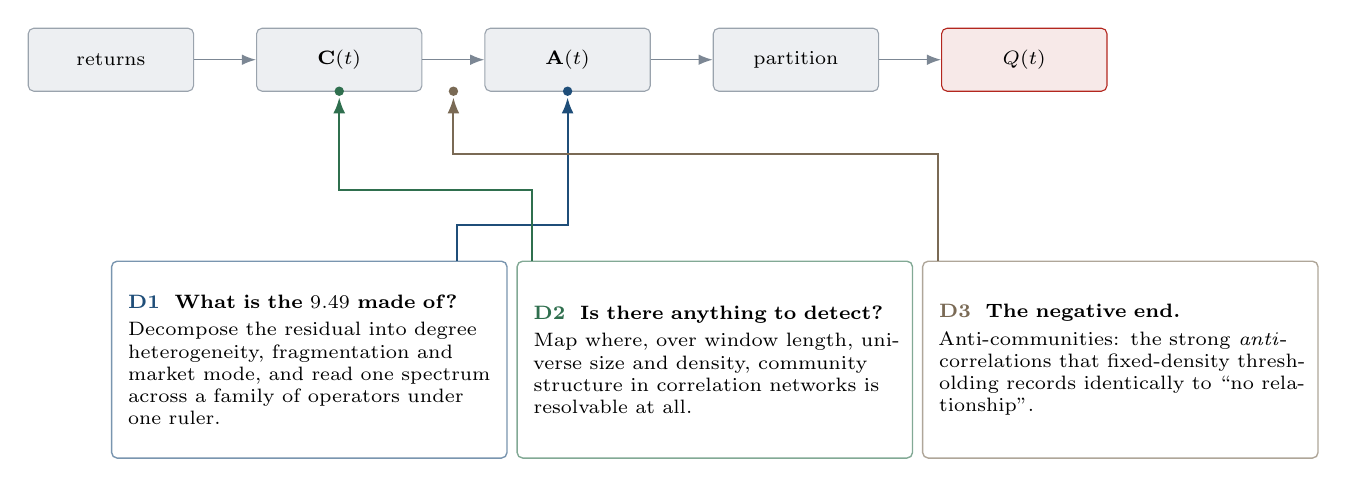
\begin{tikzpicture}[font=\small,x=1cm,y=1cm,
  st/.style={draw=Rule,line width=.4pt,rounded corners=2pt,fill=Panel,
             minimum height=8mm,minimum width=21mm,font=\scriptsize,align=center},
  dbox/.style={draw=Rule,line width=.5pt,rounded corners=2pt,fill=white,
             text width=46mm,align=left,inner sep=6pt,minimum height=25mm,
             anchor=north west,font=\scriptsize},
  ar/.style={-{Latex[length=1.8mm]},line width=.5pt,draw=Rule!130},
  up/.style={-{Latex[length=2mm]},line width=.7pt}]

\node[st] (r) at (0,0)    {returns};
\node[st] (c) at (2.9,0)  {$\Cmat(t)$};
\node[st] (a) at (5.8,0)  {$\Amat(t)$};
\node[st] (p) at (8.7,0)  {partition};
\node[st,fill=ScalC!10,draw=ScalC] (q) at (11.6,0) {$\Q(t)$};
\foreach \x/\y in {r/c,c/a,a/p,p/q} \draw[ar] (\x) -- (\y);

\node[dbox,draw=ModC!60] (d1) at (0.0,-2.55)
  {\textbf{\textcolor{ModC}{D1}\ \ What is the $9.49$ made of?}\\[2pt]
   Decompose the residual into degree heterogeneity, fragmentation and market
   mode, and read one spectrum across a family of operators under one ruler.};
\node[dbox,draw=LapC!60] (d2) at (5.15,-2.55)
  {\textbf{\textcolor{LapC}{D2}\ \ Is there anything to detect?}\\[2pt]
   Map where, over window length, universe size and density, community
   structure in correlation networks is resolvable at all.};
\node[dbox,draw=CorrC!60] (d3) at (10.3,-2.55)
  {\textbf{\textcolor{CorrC}{D3}\ \ The negative end.}\\[2pt]
   Anti-communities: the strong \emph{anti}-correlations that fixed-density
   thresholding records identically to ``no relationship''.};

% target dots
\fill[LapC]  (2.90,-0.40) circle (1.7pt);
\fill[CorrC] (4.35,-0.40) circle (1.7pt);
\fill[ModC]  (5.80,-0.40) circle (1.7pt);

% leaders, each at its own height so none overlaps another
\draw[up,ModC]  (4.40,-2.55) -- (4.40,-2.10) -- (5.80,-2.10) -- (5.80,-0.48);
\draw[up,LapC]  (5.35,-2.55) -- (5.35,-1.65) -- (2.90,-1.65) -- (2.90,-0.48);
\draw[up,CorrC] (10.50,-2.55) -- (10.50,-1.20) -- (4.35,-1.20) -- (4.35,-0.48);

\end{tikzpicture}
\caption{Where each direction attacks. D2 asks whether $\Cmat$ contains
resolvable structure in the first place; D3 concerns what the thresholding
arrow throws away; D1 concerns which operator the resulting graph should be read
through. The boxes are drawn identically on purpose.}
\label{fig:directions}
\end{figure}

\begin{table}[t]
\centering\small
\caption{The three directions in a common frame. Rows are identical questions
asked of each; nothing in the table ranks them.}
\label{tab:directions}
\renewcommand{\arraystretch}{1.12}
\begin{tabular}{@{}p{22mm}p{40mm}p{40mm}p{40mm}@{}}
\toprule
& \textbf{\textcolor{ModC}{D1}} the operator comparison
& \textbf{\textcolor{ModC}{D2}} detectability
& \textbf{\textcolor{ModC}{D3}} the negative end \\
\midrule

\textbf{The question}
& What is the $9.49$ residual made of, and which part of it carries stress
information?
& Over what region of (window, universe, density) does community structure in
correlation networks mean anything?
& Do anti-communities carry crisis information that communities do not? \\

\textbf{Evidence so far}
& $\lambda_2+\mu_1=26.41$ against $35.90$; $r=-0.187$ against $-1$
  (\S\ref{sec:duality}).
& Mean $0.70$ resolvable modes per day against Louvain's median of nine; noise
  $\Q=0.2246$ vs market $0.2215$ (\S\ref{sec:mech}).
& $\mu_N(\Bmat)$ at $0.760$, the highest-scoring new statistic
  (\S\ref{sec:disc}); $4{,}246{,}798$ discarded strong-anticorrelation
  pair-days. \\

\textbf{What exists already}
& The full spectra for all $6{,}315$ days, and the residual decomposition
  scaffolding, in \texttt{probe/duality.py}.
& The Marchenko--Pastur edge and per-day escaping-mode counts, in
  \texttt{probe/}\linebreak\texttt{spectral\_probe.py}.
& The per-day $\mu_N$ series, and the audit's count of discarded pair-days. \\

\textbf{What would be built}
& One spectrum over $\Amat$, $\Lap$, normalised $\Lap$, $\Bmat$, normalised
  $\Bmat$, and MacMahon--Garlaschelli's threshold-free correlation modularity,
  under the ruler of \S\ref{sec:ruler}.
& A grid over $\Delta t$, $N$ and density, benchmarked against both the MP edge
  and the Nadakuditi--Newman detectability threshold; plus a deterministic
  Louvain-free community count.
& The anti-correlation series reconstructed and scored; $\mu_N$ re-scored with
  the market mode projected out. \\

\textbf{Currently untested}
& Whether the decomposition is stable across network constructions, not just
  Silva's.
& Whether any configuration used in the literature falls inside the resolvable
  region.
& Whether $\mu_N$ survives removing the market mode --- it borrows $0.680$ from
  it on the scored series (\S\ref{sec:caveats}). A two-day check. \\

\textbf{What could go wrong}
& The gap may turn out to be dominated by fragmentation, i.e.\ an artifact of
  thresholding rather than a market property.
& If essentially no configuration in the literature is inside the region, the
  contribution is purely negative --- publishable, but harder to place.
& If $\mu_N$ does not survive market-mode removal, the result folds back into
  D1 as one component of the residual. \\
\bottomrule
\end{tabular}
\end{table}

One factual note that belongs with D3 rather than with any ranking: the
discarded anti-correlation series \emph{collapses to near zero from roughly
2003 and never recovers}, which sits directly beside the unexplained 2002 break
that Silva et al.\ report and list as future work. Whether the two are connected
is untested.

\appendix
\section{Where every number comes from}

Nothing in this document is retyped from a figure. Each row below names the
script that produces the value and the file it is stored in; all paths are
relative to the repository root. The probe imports Silva's replication's own
\texttt{utils/crisis\_dates.py}, \texttt{net/construct.py} and scoring
conventions unchanged.

\begin{center}
\small
\begin{tabular}{@{}lll@{}}
\toprule
\textbf{Numbers} & \textbf{Produced by} & \textbf{Stored in} \\
\midrule
All 16 AUCs (Table~\ref{tab:leaderboard}) & \texttt{probe/spectral\_probe.py} & \texttt{probe/spectral\_probe\_auc.json} \\
$\lambda_2$ on the largest component & \texttt{probe/duality.py} & \texttt{probe/duality\_auc.json} \\
Per-day spectra, $6{,}315\times16$ & \texttt{probe/spectral\_probe.py} & \texttt{probe/spectral\_probe.parquet} \\
Residual, $\operatorname{corr}(\lambda_2,\mu_1)$ (Table~\ref{tab:duality}) & \texttt{probe/duality.py} & the parquet above \\
Escaping-mode counts (Figure~\ref{fig:mp}) & \texttt{probe/spectral\_probe.py} & the parquet above \\
In/out-of-sample AUCs (Table~\ref{tab:oos}) & \texttt{probe/incremental.py} & \texttt{probe/incremental\_auc.json} \\
Louvain stability, noise-control $\Q$ & Silva replication, phases 3--8 & \texttt{results/phase8\_extensions.json} \\
Discarded anticorrelated pair-days & Silva replication, phase 2 & \texttt{PITFALLS.md} (A8) \\
\bottomrule
\end{tabular}
\end{center}

\noindent All of it is re-checked by \texttt{reports/probe/check\_numbers.py},
which recomputes every value quoted here from those files and fails loudly on
any mismatch.

\vspace{3mm}
\noindent\textbf{Reproducing.} The probe needs the replication's derived
artifacts (\texttt{data/edges.npy}, \texttt{data/returns.npy},
\texttt{results/series/*.parquet}), which are gitignored as rebuildable;
regenerate them with \texttt{python run\_phases.py 1 3} inside
\texttt{paper3\_market\_modularity/} first. Silva's pipeline needs
\texttt{python-igraph}.

\vspace{3mm}
\noindent{\footnotesize\textbf{Outside references used above.} Kritzman et al.\
2011 (absorption ratio, the baseline to beat); Laloux et al.\ and Plerou et al.\
1999 (RMT precursors); Newman 2006 (the modularity matrix); Fasino \& Tudisco
2014/2016/2017 (modularity spectrum, community counts, anti-communities);
Nadakuditi \& Newman 2012 (detectability); MacMahon \& Garlaschelli 2015 (the
correlation-specific null Silva et al.\ needed and did not use); Masuda et al.,
\emph{Physics Reports} 2025 (the ``beyond thresholding'' review); Kang et al.\
2025 (largest Laplacian gap). Papers replicated: arXiv:2005.09958 (Cardoso \&
Palomar), arXiv:1706.03161 (TICC), arXiv:1501.05040 (Silva et al.).
\textcolor{BadRed}{This list was assembled largely with Claude and I have not
read most of these papers in full --- see the aside in \S1. It is a working set
of pointers, not a literature review.} \textcolor{BadRed}{Two Laplacian-energy papers (\emph{Eur.\ J.\ Finance} 29(9)
2023; \emph{Int.\ Rev.\ Econ.\ Finance} 2025) have unverified author lists and
must not be cited as-is.}\par}

\end{document}
